\clearpage
\thispagestyle{empty}
\null
\newpage

\cleardoublepage
\phantomsection
% \pdfbookmark[1]{Validation expérimentale de la méthode}{Validation expérimentale de la méthode}
\markboth{\spacedlowsmallcaps{Validation expérimentale de la méthode}}{\spacedlowsmallcaps{Validation expérimentale de la méthode}}
\part{Validation expérimentale de la méthode}
\label{part:experimentation}

\clearpage
\thispagestyle{empty}
\null
\newpage

\chapter*{Introduction}
\addcontentsline{toc}{chapter}{\textbf{Introduction}}

\noindent
Cette partie vise à démontrer l'applicabilité et la pertinence de la méthode \acn{MAMAD} dans l'ensemble de ses activités ou une partie d'entre elles dans différents contextes de conception de systèmes multi-agents. Pour cela, nous avons développé une plateforme dédiée, \acn{CybMASDE}, qui implémente l'ensemble du pipeline proposé (modélisation, apprentissage, analyse, transfert) de manière modulaire et reproductible.

\medskip

\noindent
Comme illustré en \autoref{fig:organisation_manuscrit_partie_4}, dans un premier temps, nous décrivons en détail l'environnement expérimental, les outils logiciels et matériels mobilisés, ainsi que les environnements de test retenus. Nous présentons également les spécifications organisationnelles associées à chaque environnement, ainsi que les métriques d'évaluation permettant de valider les performances de la méthode.

\medskip

\noindent
Dans un second temps, nous analysons les résultats obtenus afin de répondre aux objectifs de recherche identifiés dans la partie précédente. Cela inclut une évaluation de l'efficacité de la méthode, de sa capacité d'automatisation, de l'adéquation des politiques apprises avec les contraintes organisationnelles, ainsi que de leur explicabilité.

\medskip

\noindent
Cette étude expérimentale nous permettra de mieux cerner les atouts et les limites de la méthode \acn{MAMAD}, et de dégager des perspectives d'amélioration pour une automatisation encore plus poussée de la conception organisationnelle en \acn{MARL}.



\begin{figure}[h!]
  \centering
  \resizebox{0.8\linewidth}{!}{%
    \begin{tikzpicture}[
        chapter/.style={draw, fill=blue!10, thick, minimum width=9cm, minimum height=1.2cm, text centered, font=\bfseries},
        section/.style={draw, fill=blue!5, thick, minimum width=8cm, minimum height=1cm, text centered, font=\small},
        arrow/.style={-Latex, thick},
        node distance=0.4cm,
        annotated/.style={above,font=\small\itshape, inner sep=1pt, yshift=0.8cm, xshift=-8cm}
    ]

    % Chapitre 11 : Implémentation et outils
    \node[chapter] (ch11) {\parbox{10cm}{Chapitre 11 : CybMASDE : Un framework supportant MAMAD}};
    \node[section, below=1cm of ch11, xshift=-2cm] (ch11s1) {Intégration des différentes contributions};

    \draw[arrow] ($ (ch11.south) + (4.0,0) $) -- ++(0,0) |- (ch11s1.east) node[annotated] {Architecture logicielle modulaire au cœur du framework.};

    % Chapitre 12 : Cadre expérimental
    \node[chapter, below=1cm of ch11s1, xshift=2cm] (ch12) {\parbox{10cm}{Chapitre 12 : Cadre expérimental et d'évaluation}};
    \node[section, below=1cm of ch12, xshift=-2cm] (ch12s1) {Description des ensembles d'environnements et d'algorithmes considérés};
    \node[section, below=1cm of ch12s1] (ch12s2) {Conditions de reproductibilité};
    \node[section, below=1cm of ch12s2] (ch12s3) {Baselines expérimentales};
    \node[section, below=1cm of ch12s3] (ch12s4) {Grille d'évaluation};
    \node[section, below=1cm of ch12s4] (ch12s5) {Protocole d'experimentation et d'évaluation};

    \draw[arrow] ($ (ch12.south) + (4.0,0) $) -- ++(0,0) |- (ch12s1.east) node[annotated] {Définition des briques fondatrices pour l'experimentation.};
    \draw[arrow] ($ (ch12.south) + (4.0,0) $) -- ++(0,0) |- (ch12s2.east) node[annotated] {Résumé des conditions de reproduction expérimentales};
    \draw[arrow] ($ (ch12.south) + (4.0,0) $) -- ++(0,0) |- (ch12s3.east) node[annotated] {Définition les différentes expérimentations};
    \draw[arrow] ($ (ch12.south) + (4.0,0) $) -- ++(0,0) |- (ch12s4.east) node[annotated] {Définition un cadre commun pour l'évaluation};
    \draw[arrow] ($ (ch12.south) + (4.0,0) $) -- ++(0,0) |- (ch12s5.east) node[annotated] {Assemblage des éléments pour définir un protocole};

    % Chapitre 13 : Études de cas
    \node[chapter, below=1cm of ch12s5, xshift=2cm] (ch13) {\parbox{10cm}{Chapitre 13 : Études de cas}};
    \node[section, below=1cm of ch13, xshift=-2cm] (ch13s1) {Expérimentations sur les environnements non-orientés Cyberdéfense};
    \node[section, below=1cm of ch13s1] (ch13s2) {Expérimentations sur l'environnement Company infrastructure};
    \node[section, below=1cm of ch13s2] (ch13s3) {Expérimentations sur l'environnement Microservices Kubernetes};
    \node[section, below=1cm of ch13s3] (ch13s4) {Expérimentations sur l'environnement Drone Swarm};

    \draw[arrow] ($ (ch13.south) + (4.0,0) $) -- ++(0,0) |- (ch13s1.east) node[annotated] {};
    \draw[arrow] ($ (ch13.south) + (4.0,0) $) -- ++(0,0) |- (ch13s2.east) node[annotated] {};
    \draw[arrow] ($ (ch13.south) + (4.0,0) $) -- ++(0,0) |- (ch13s3.east) node[annotated] {};
    \draw[arrow] ($ (ch13.south) + (4.0,0) $) -- ++(0,0) |- (ch13s4.east) node[annotated] {};

    % Chapitre 14 : Résultats et synthèse
    \node[chapter, below=1cm of ch13s4, xshift=2cm] (ch14) {\parbox{10cm}{Chapitre 14 : Résultats expérimentaux et analyse}};
    \node[section, below=1cm of ch14, xshift=-2cm] (ch14s1) {Résultats et discussion des environnements non-orientés Cyberdéfense};
    \node[section, below=1cm of ch14s1] (ch14s2) {Résultats et discussion de l'environnement Company Infrastructure};
    \node[section, below=1cm of ch14s2] (ch14s3) {Résultats et discussion de l'environnement Microservices Kubernetes};
    \node[section, below=1cm of ch14s3] (ch14s4) {Résultats et discussion de l'environnement Drone Swarm};

    \draw[arrow] ($ (ch14.south) + (4.0,0) $) -- ++(0,0) |- (ch14s1.east) node[annotated] {};
    \draw[arrow] ($ (ch14.south) + (4.0,0) $) -- ++(0,0) |- (ch14s2.east) node[annotated] {};
    \draw[arrow] ($ (ch14.south) + (4.0,0) $) -- ++(0,0) |- (ch14s3.east) node[annotated] {};
    \draw[arrow] ($ (ch14.south) + (4.0,0) $) -- ++(0,0) |- (ch14s4.east) node[annotated] {};

    % Transitions entre chapitres
    \draw[arrow] ($ (ch11.south) + (4.5,0) $) -- ($ (ch12.north) + (4.5,0) $) node[annotated, yshift=-0.5cm] {L'outil étant en place, nous définissons le protocole pour l'évaluer.};
    \draw[arrow] ($ (ch12.south) + (4.5,0) $) -- ($ (ch13.north) + (4.5,0) $) node[annotated, yshift=-0.5cm] {Le protocole est appliqué à différents environnements.};
    \draw[arrow] ($ (ch13.south) + (4.5,0) $) -- ($ (ch14.north) + (4.5,0) $) node[annotated, yshift=-0.5cm] {Les résultats sont analysés pour valider la méthode.};

\end{tikzpicture}

  }
  \caption{Structure de la Partie IV~: Cadre expérimental et analyse des résultats}
  \label{fig:organisation_manuscrit_partie_4}
\end{figure}

\clearpage
\thispagestyle{empty}
\null
\newpage

\chapter{CybMASDE: Un framework supportant MAMAD}
\label{sec:cybmasde}

Pour soutenir la mise en œuvre modulaire et reproductible de la méthode \acn{MAMAD}, nous avons conçu la plateforme \acn{CybMASDE}~\footnotemark[2]. Elle orchestre les activités de modélisation, d'entraînement, d'analyse et de déploiement de \acn{SMA} fondés sur le cadre MOISE+MARL.

\footnotetext[2]{Code source et documentation disponibles à \url{https://github.com/julien6/CybMASDE}}

Le module de modélisation construit un modèle de prédiction d'observations conjointes (\acparen{JOPM}) via PyTorch, avec des dynamiques \acn{LSTM} entraînées à partir des historiques réels $\mathcal{D}_{H^j}$. Les observations sont compressées à l'aide d'encodeurs \acn{VAE} (dimensions latentes entre 16 et 64), tandis que les actions sont encodées via des \acn{MLP}. Le \acn{LSTM} utilise des tailles cachées de 64 ou 128, et est optimisé par Adam (taux d'apprentissage entre $1 \times 10^{-4}$ et $5 \times 10^{-4}$). La fonction de récompense $R^j_H$ est dérivée manuellement de $\mathcal{G}_{\text{inf}}$ et les contraintes organisationnelles $\mathcal{C}_{\text{inf}}$ sont formalisées en spécifications MOISE+MARL $\mathcal{MM}$ via l'API \acn{MMA}.

L'entraînement est effectué avec MARLlib~\cite{hu2022marllib}, qui prend en charge \acn{MAPPO}, \acn{MADDPG}, \acn{QMix}, \acn{IQL}, \acn{VDN} et \acn{ROMA}. Les contraintes MOISE+MARL sont appliquées via du masquage d'actions par rôle et du shaping de récompense. L'apprentissage utilise Ray RLlib avec un taux d'apprentissage dans $[1e^{-4}, 5e^{-4}]$, un facteur d'actualisation dans $[0.9, 0.99]$, une valeur de clip \acn{PPO} dans $[0.1, 0.3]$ et des tailles de batchs dans $\{64, 128\}$, avec des politiques implémentées par \acn{MLP}s de 64 à 256 neurones.

L'analyse implémente la méthode Auto-TEMM, une extension de \acn{TEMM} avec optimisation complète des hyperparamètres via Optuna. Les trajectoires sont regroupées par clustering hiérarchique selon des métriques (\acparen{DTW}, \acparen{LCS}...), avec optimisation de la distance minimale intra-cluster. Un balayage de la représentativité (de 0.0 à 1.0) est effectué pour identifier celle qui minimise le temps de convergence vers une récompense cible (par défaut~: 3.5\%). Le "adéquation  organisationnel" est ensuite calculé comme la moyenne des composantes \acn{SOF} (structurelle) et \acn{FOF} (fonctionnelle) issues des variances intra-cluster.

Le module de transfert assure le déploiement continu des politiques $\pi^j_{\text{latest}}$ dans des environnements réels ou simulés via PettingZoo ou des API spécifiques. Une fois un seuil atteint (ex. 512 étapes), une nouvelle boucle de modélisation-entraînement-analyse est déclenchée.

Ainsi, \acn{CybMASDE} constitue une chaîne d'outils complète et extensible pour exécuter la méthode \acn{MAMAD}, en intégrant simulation, apprentissage \acn{MARL}, inférence organisationnelle et déploiement dans un même environnement.

% \section{Intégration des \textit{World Models} Multi-Agents}


\section{Intégration du framework environnemental MCAS}

\noindent
Les travaux potentiels pour mettre en œuvre notre modèle comprennent~: NeSSi2~\cite{DGrunewald2011}, une plateforme de simulation basée sur des agents visant à modéliser uniquement la description au niveau des paquets d'un système en réseau et les effets des attaques DDoS~; et Kotenko et al.~\cite{IKotenko2007}, qui s'appuie sur OMNet++~\cite{Varga2010} pour modéliser et simuler des agents de cyberdéfense coopératifs contre les attaques réseau, en combinant la simulation d'événements discrets, l'approche multi-agents et la simulation au niveau des paquets des protocoles réseau.
% De plus, pour pallier le manque de réalisme, des émulateurs utilisant des machines virtuelles et intégrés à des outils offensifs ont été développés, tels que DCAFE~\cite{GRush2014} et SVED~\cite{HHannes2016}.
Cependant, parmi ceux-ci, aucun ne peut pleinement répondre à la fois à la prise en compte d'un environnement cyber multi-agents pour un modèle Dec-POMDP
%et le besoin d'accessibilité du code (code source ouvert).

Cependant, nous avons identifié des simulateurs d'événements discrets avec un seul cyberattaquant, tels que CYST\cite{drasar_session-level_2020} ou CyberBattleSim~\cite{cyberbattlesim}, qui fournissent tous deux une simulation de réseau et une approche d'évaluation adaptées à la mise en œuvre de notre modèle, car leurs modèles sous-jacents peuvent être étendus à plusieurs agents. Inspirés par ces approches, nous avons utilisé \textit{PettingZoo}~\cite{terry2020pettingzoo} comme plateforme fondamentale pour implémenter notre modèle Dec-POMDP sur lequel nous avons cherché à implémenter un réseau simulé. \textit{PettingZoo} fournit un cadre dans lequel le concepteur dispose d'outils pour faciliter la mise en œuvre de l'espace d'observations, des actions, de la gestion des agents à chaque tour et des récompenses associées.

% \begin{figure}
%      \centering
%      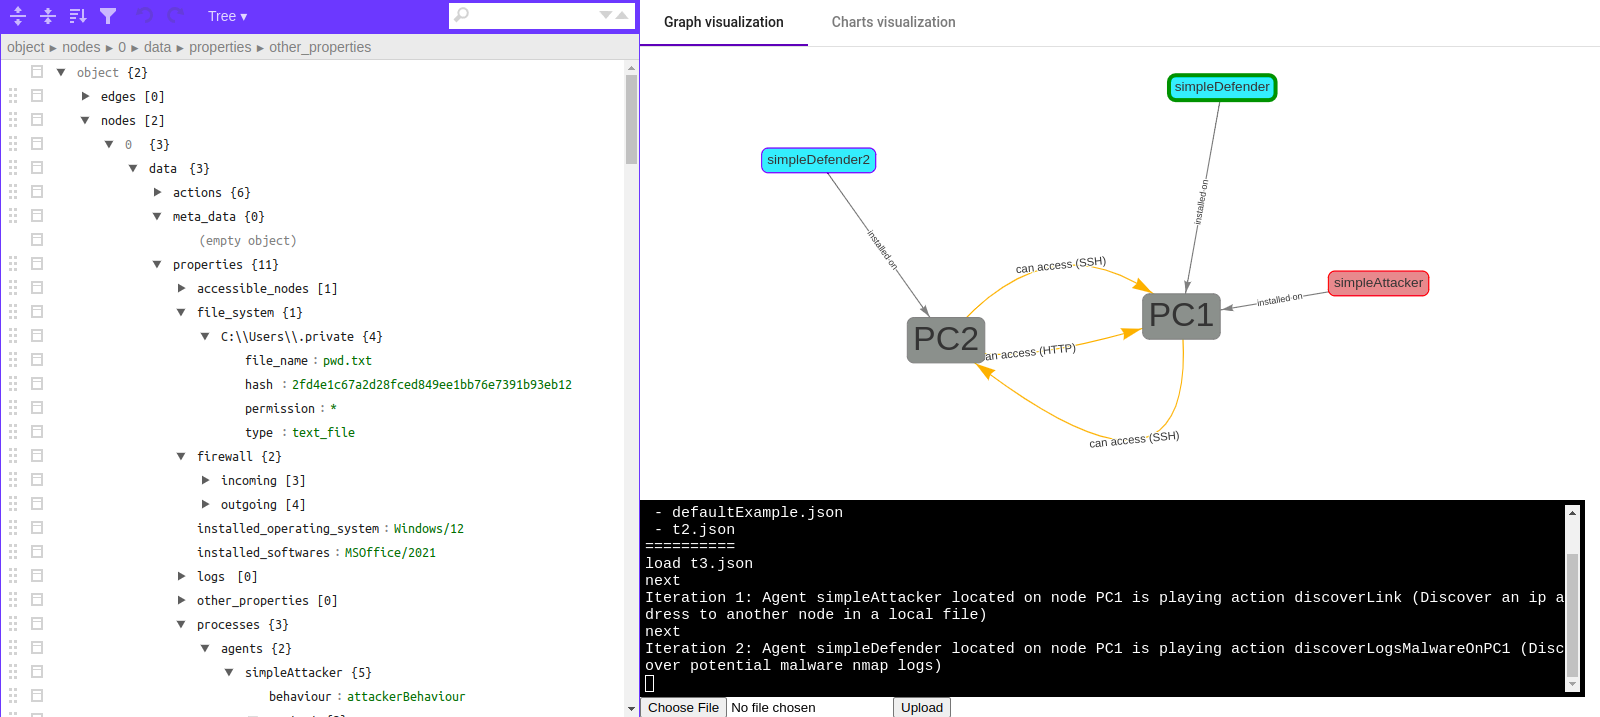
\includegraphics[width=\linewidth]{figures/interface_MCAS.png}
%      \caption{Aperçu de l'interface du simulateur}
%      \label{fig:simulator_interface}
% \end{figure}

Le développement de notre modèle a abouti au simulateur \textquote{Multi Cyber Agent Simulator} (MCAS)~\cite{MCASWebsite}. Dans son état actuel, ce simulateur permet de charger/enregistrer un fichier \textit{json} décrivant les propriétés des nœuds et les actions de l'environnement, ainsi que les agents définis et leurs comportements~; il permet également de lancer l'exécution des agents de cet environnement en mode tour à tour via le terminal. Il est possible de visualiser les propriétés de l'environnement en temps réel et de représenter l'environnement sous forme de graphique. Des métriques sont également affichées.



\section{Intégration du framework MOISE+MARL}

Nous avons développé une implémentation du cadre MOISE+MARL appelée \textquote{MMA}~\hyperref[fn:github]{\footnotemark[2]} (API MOISE+MARL), qui est une API Python intégrant tous les ensembles et relations théoriques afin de minimiser les interactions avec l'utilisateur. MMA utilise une approche orientée objet, structurant le modèle $\mathcal{M}OISE^+$ en classes de données imbriquées, avec la classe « Moise » à la racine, permettant aux utilisateurs de définir des spécifications organisationnelles, telles que les rôles, les objectifs et les autorisations.

Pour prendre en charge les environnements Dec-POMDP, nous avons utilisé la bibliothèque \textit{PettingZoo} \cite{terry2020pettingzoo}, qui fournit une API standard pour les systèmes multi-agents et garantit l'interopérabilité entre différents environnements, à l'instar du framework Gymnasium \cite{kwiatkowski2024}. MMA intègre un dictionnaire pour le mappage des étiquettes d'observation/action ($l$), que les utilisateurs peuvent personnaliser, et prend également en charge les modèles de trajectoire (TP) pour faciliter la définition et la correspondance des modèles.

Chaque type de guide de contrainte, comme $rag$, $rrg$ et $grg$, est implémenté dans une classe distincte. Les utilisateurs peuvent définir ces guides à l'aide de fonctions personnalisées ou de règles JSON~; par exemple, $rag$ peut être instancié en associant une paire $\langle \text{TP, dernière observation} \rangle$ aux actions attendues, tandis que $grg$ peut appliquer des bonus en fonction de TP spécifiques. La classe globale « MMA » intègre ces guides avec des relations définies par l'utilisateur, telles que la liaison d'un agent à un rôle ($ar$) ou l'association d'un rôle à $rrg$ et $rag$, en incorporant les spécifications organisationnelles définies dans la structure $\mathcal{M}OISE^+$.

Une fois configuré, l'objet MMA est utilisé pour encapsuler l'environnement avec un wrapper \textit{PettingZoo}. Ce wrapper applique des masques d'action et modifie les récompenses à chaque étape, garantissant que les agents respectent les spécifications organisationnelles tout au long de la formation. MMA intègre également \textit{MARLlib} \cite{hu2021marlib}, qui donne accès à des algorithmes MARL de pointe, permettant ainsi d'exécuter l'entraînement sur un cluster informatique haute performance.

Après l'entraînement, la méthode TEMM est utilisée, en utilisant des hyperparamètres optimisés manuellement pour déduire les rôles et les objectifs implicites grâce à un regroupement hiérarchique et à la méthode K-means. Cette analyse génère des résultats visuels, tels que des dendrogrammes pour les rôles et des graphiques de transition d'observation conjointe pour les objectifs. Les rôles et les objectifs implicites qui en résultent peuvent être exportés sous forme de trajectoires JSON, offrant une vue structurée des comportements organisationnels déduits.




\clearpage
\thispagestyle{empty}
\null
\newpage

\chapter{Protocole expérimental}
\label{chap:experimental_protocol}

Ce chapitre définit un protocole expérimental générique, applicable à tous les cas d'étude présentés dans ce chapitre.
L'objectif est de fournir un \textit{canevas} que chaque scénario peut instancier en précisant ses choix propres.
Ce protocole s'appuie sur la méthode \acn{MAMAD}, la taxonomie des activités et sous-activités présentée en \autoref{tab:mamad_taxonomy}, et les critères d'évaluation définis précédemment.

\section{Cadre expérimental général}
\label{sec:generic_experimental_framework}

Le protocole couvre, au besoin, l’entièreté du cycle de vie MAMAD pour un \acn{SMA} : de la modélisation de l’environnement (jumeau numérique) à l’entraînement, l’analyse organisationnelle et le transfert des politiques. Il distingue deux catégories d’éléments, afin d’éviter toute redondance dans les études de cas du \autoref{chap:case_studies} :
\begin{itemize}
  \item \textbf{Constantes} — Choix méthodologiques communs (familles d’algorithmes MARL, format des spécifications organisationnelles, critères et métriques de base, ressources matérielles, procédures d’évaluation).
  \item \textbf{Variables} — Paramètres et composants \textit{spécifiques} à un cas d’étude (environnement cible, sous-activités MAMAD activées, hyperparamètres surchargés, baselines additionnelles, perturbations).
\end{itemize}

\paragraph{Algorithmes MARL de référence}
Le protocole prend en charge un panel d’algorithmes représentatifs des grandes familles, afin de couvrir des biais inductifs variés :
\begin{itemize}
  \item \textbf{Value-based} (ex.~\texttt{QMIX}) : décomposition de la valeur conjointe pour la coopération.
  \item \textbf{Policy-based} (ex.~\texttt{MADDPG}) : politiques déterministes avec apprentissage centralisé/exécution décentralisée.
  \item \textbf{Actor--Critic} (ex.~\texttt{MAPPO}) : optimisation robuste de politiques conjointes dans des dynamiques complexes.
\end{itemize}
\textit{Principe~:} sauf mention contraire dans une étude de cas, ces familles servent de \textbf{références communes}. Chaque scénario peut restreindre le panel (p.~ex. garder MAPPO uniquement) pour des raisons techniques, tout en conservant la comparabilité via les baselines (\autoref{par:baselines}).

\paragraph{Spécifications organisationnelles}
Lorsque des contraintes organisationnelles sont utilisées, elles sont formalisées avec \acn{MOISE+MARL} et décrivent~:
\begin{itemize}
  \item les \textbf{rôles} (hiérarchie et héritage)~;
  \item les \textbf{missions} et \textbf{objectifs} intermédiaires (plans, jalons)~;
  \item les \textbf{spécifications déontiques} (permissions, obligations, interdictions).
\end{itemize}
Les entraînements \textbf{non contraints} sont représentés par un \textit{ensemble vide} de spécifications (cas \acn{TRN-UNC}). Les modes d’intégration des contraintes utilisés dans le protocole sont explicites et communs à tous les scénarios~:
\begin{enumerate*}[label=\roman*)]
  \item \textit{penalize} (pénalisation dans la récompense),
  \item \textit{correct} (correction d’action),
  \item \textit{correct\_policy} (politique composite contraignante)
\end{enumerate*}.
Sauf précision contraire, le degré de \textit{dureté} des contraintes est fixé à~1 pour les mesures principales, avec ablation optionnelle (dureté~$\in[0,1]$).

\paragraph{Activités et sous-activités MAMAD}
Chaque cas d’étude \textbf{déclare explicitement} les activités et sous-activités utilisées au moyen des acronymes de la taxonomie (p.~ex.~\acn{MOD-AUT}, \acn{TRN-CON}, \acn{ANL-AUT}, \acn{TRF-AUT}). Cette déclaration sert d’\textit{en-tête} standardisé de l’étude de cas et permet d’identifier immédiatement le \textit{chemin méthodologique} activé.

\paragraph{Critères communs de validation}
Les expériences sont évaluées suivant les 8 critères principaux définis en \autoref{sec:critere_hierarchie}. Chaque critère est relié à des métriques opérationnelles et à une ou plusieurs activités MAMAD. Les études de cas sélectionnent un \textit{sous-ensemble ciblé} de critères en fonction de leurs objectifs, mais conservent la sémantique commune pour la comparaison inter-scénarios.

\paragraph{Métriques communes retenues}
Le protocole impose un \textit{noyau} de métriques :
\begin{itemize}
  \item \textbf{Performance}~: récompense moyenne (par épisode / par fenêtre), écart-type (\emph{Std Reward})~;
  \item \textbf{Organisation}~: \acn{OF} (global), \acn{SOF} (structurel), \acn{FOF} (fonctionnel) — issus de \acn{TEMM}~;
  \item \textbf{Robustesse et scalabilité}~: taux de convergence (épisodes jusqu’au seuil), maintien de performance sous perturbations (bruit, pannes, adversaires), sensibilité au nombre d’agents.
\end{itemize}
Les scénarios peuvent \textit{ajouter} des métriques spécifiques (p.~ex. \% de drones infectés, \% d’attaques réussies) tant qu’elles sont reliées à un critère principal.

\begin{table}[h!]
  \centering
  \caption{Lien entre critères, métriques et activités MAMAD}
  {%

    \footnotesize
    \begin{tabular}{p{3.2cm}p{4.2cm}p{5.1cm}}
      \hline
      \textbf{Critère}            & \textbf{Métriques}                                    & \textbf{Activités concernées} \\
      \hline
      Performance globale         & Récompense moyenne, Std Reward                        & \acn{TRN}                     \\
      Cohérence organisationnelle & \acn{OF}, \acn{SOF}, \acn{FOF}                        & \acn{ANL}                     \\
      Vitesse de convergence      & \#~épisodes pour atteindre un seuil                   & \acn{TRN}                     \\
      Robustesse                  & Écart de performance sous perturbations               & \acn{TRN}, \acn{ANL}          \\
      Scalabilité                 & Variation des perfs vs nombre d’agents / taille tâche & \acn{MOD}, \acn{TRN}          \\
      Qualité de la modélisation  & Précision de prédiction du jumeau numérique           & \acn{MOD}                     \\
      Impact du guidage           & Diff. des métriques avec/sans MOISE+MARL              & \acn{TRN}, \acn{ANL}          \\
      Transférabilité             & Maintien des perfs après transfert (\acn{TRF})        & \acn{TRF}                     \\
      \hline
    \end{tabular}
  }
  \label{tab:criteria_metrics}
\end{table}

\paragraph{Conditions expérimentales matérielles}
\label{par:compute_conditions}
Les expériences sont réalisées sur un \textbf{cluster HPC académique}. Sauf mention contraire, les constantes suivantes s’appliquent à tous les scénarios~:
\begin{itemize}
  \item \textbf{Accélérateurs}~: NVIDIA A100 / V100, AMD MI210.
  \item \textbf{Frameworks DL}~: PyTorch et TensorFlow (implémentations MARLlib/MAPPO, etc.).
  \item \textbf{Optimisation d’hyperparamètres}~: \textbf{Optuna} pour LR, rapports exploration/exploitation, tailles de réseaux, avec \textit{samplers} TPE ; espace de recherche standardisé par famille d’algorithmes.
  \item \textbf{Parallélisme}~: \underline{5 exécutions indépendantes} par condition (algorithme $\times$ environnement $\times$ mode de contrainte) pour robustesse statistique.
  \item \textbf{OS et libs}~: Linux 64-bit, CUDA/cuDNN ou ROCm selon GPU ; versions figées par fichier d’environnement (conda/pip) commun.
\end{itemize}
Les études de cas n’ont \textbf{pas} à répéter ces éléments ; seules les \textit{déviations} (p.~ex. nombre de runs, GPU spécifique) doivent être précisées.

\paragraph{Gestion des hyperparamètres (par défaut et surcharges)}
Par défaut, chaque couple \{algorithme, environnement\} est initialisé avec un \textit{profil standard} (LR, tailles MLP, horizon, batch) issu de banques MARLlib et/ou d’expériences préliminaires. \textbf{Optuna} peut être activé pour une passe d’HPO \textit{contrôlée} (\#~d’essais borné, mêmes priorités d’espace de recherche entre scénarios), puis le meilleur \textit{trial} est \textbf{rejoué 5 fois} pour agrégation des résultats. Les scénarios peuvent :
\begin{enumerate*}[label=\alph*)]
  \item accepter les valeurs par défaut,
  \item restreindre l’HPO,
  \item surcharger explicitement certains hyperparamètres (justification requise).
\end{enumerate*}

\paragraph{Baselines}
\label{par:baselines}
Le protocole définit des baselines communes~:
\begin{itemize}
  \item \textbf{RB} — MARL \textit{sans} contraintes organisationnelles (\acn{TRN-UNC}).
  \item \textbf{OB} — MARL \textit{avec} contraintes MOISE+MARL définies manuellement (rôles/missions minimales mais fonctionnelles).
  \item \textbf{MB} — \acn{MAMAD} avec \textit{inférence} (TEMM/Auto-TEMM) + guidage (MOISE+MARL) quand applicable.
  \item \textbf{Ablation optionnelle} -- AGR+MARL (rôles sans objectifs intermédiaires) pour isoler l’apport des objectifs.
\end{itemize}
Chaque étude de cas indique quelles baselines sont pertinentes et, le cas échéant, lesquelles sont omises (avec raison).

\paragraph{Procédure d’évaluation et reproductibilité}
\begin{itemize}
  \item \textbf{Répétitions}~: 5 runs indépendants par condition, \textit{seeds} distinctes mais consignées.
  \item \textbf{Fenêtrage}~: métriques \textit{on-policy} (pendant l’entraînement) et \textit{off-policy} (évaluations figées) agrégées par fenêtres glissantes (taille fixée globalement).
  \item \textbf{Seuils de validation}~: $\texttt{org\_fit}_{min}$, $\overline{r}_{min}$, $\sigma_{max}$ fixés globalement (valeurs par défaut) et réutilisés entre scénarios ; toute modification est reportée en étude de cas.
  \item \textbf{Tests statistiques}~: comparaison des moyennes (t-test ou test non paramétrique selon normalité), IC à 95\%, correction de multiplicité si nécessaire.
  \item \textbf{Arrêt anticipé}~: \textit{early stopping} autorisé sur plateau de performance (critère commun), avec reprise à partir des derniers checkpoints valides.
  \item \textbf{Traçabilité}~: versionnement des configs (\texttt{.yaml}), des scripts, des commits, et \textit{hash} des datasets synthétisés (traces).
\end{itemize}

\paragraph{Paramètres communs par défaut et surcharges par scénario}
\begin{table}[h!]
  \centering
  \caption{Paramètres communs (défauts) et points de surcharge par scénario}
  {%

    \footnotesize
    \begin{tabular}{p{5.2cm}p{7.2cm}}
      \hline
      \textbf{Paramètre (défaut)}               & \textbf{Surcharge possible en étude de cas}           \\
      \hline
      Algorithmes évalués (QMIX, MADDPG, MAPPO) & Restreindre à un sous-ensemble avec justification     \\
      \# runs indépendants (5)                  & Augmenter/Diminuer (coût $\leftrightarrow$ précision) \\
      Intégration contrainte (correct\_policy)  & Basculer vers penalize/correct pour ablations         \\
      Dureté des contraintes (1.0)              & Balaye $\in \{0, 0.5, 1\}$                            \\
      Optuna (budget fixe d’essais)             & Désactiver, restreindre, ou étendre le budget         \\
      Fenêtre d’agrégation (taille $w$)         & Ajuster $w$ pour dynamiques rapides/lentes            \\
      Seuils de validation globaux              & Ajuster à la difficulté de l’env. (reporter valeurs)  \\
      \hline
    \end{tabular}
  }
\end{table}

Chaque étude de cas du chapitre suiviant se limite à \textbf{instancier} ce cadre en complétant le gabarit tabulaire (activités/sous-activités MAMAD, algorithmes retenus, spécifications organisationnelles, critères cibles, métriques associées, baselines, particularités de modélisation). Les \textit{protocoles}, \textit{conditions matérielles} et \textit{procédures d’évaluation} ne sont \textbf{pas} répétés : seules les \textit{déviations} au présent cadre sont mentionnées.


\section{Gabarit d’instanciation pour un cas d’étude}
Chaque scénario du chapitre 13 remplit le tableau suivant pour spécifier les choix particuliers :

\begin{table}[h!]
  \centering
  \caption{Gabarit d’instanciation du protocole expérimental pour un cas d’étude}
  \label{tab:case_protocol_instance}
  \renewcommand{\arraystretch}{1.2}
  {%

    \footnotesize
    \begin{tabular}{p{5cm}p{8.5cm}}
      \hline
      \textbf{Élément}                                  & \textbf{Valeur instanciée pour le scénario}                                                                                                                                                                              \\
      \hline
      \textbf{Nom du scénario}                          & Nom court et description synthétique de l’environnement étudié.                                                                                                                                                          \\

      \textbf{Activités / sous-activités MAMAD}         & Liste des acronymes selon la taxonomie (ex.~\acn{MOD-AUT}, \acn{TRN-CON}, \acn{ANL-AUT}, \acn{TRF-AUT}).                                                                                                                 \\

      \textbf{Objectifs expérimentaux spécifiques}      & Liste des objectifs ciblés, en lien explicite avec les critères principaux (\autoref{sec:critere_hierarchie}). Exemple : \textit{évaluer l’impact du guidage organisationnel sur la vitesse de convergence (critère~4)}. \\

      \textbf{Algorithmes MARL utilisés}                & Sélection parmi les algorithmes de référence (\texttt{QMIX}, \texttt{MADDPG}, \texttt{MAPPO}) ou autres algorithmes si justification.                                                                                    \\

      \textbf{Spécifications organisationnelles}        & Description ou référence à la définition MOISE+MARL utilisée (rôles, missions, contraintes). Indiquer si \texttt{ensemble vide} pour un entraînement non contraint.                                                      \\

      \textbf{Critères principaux ciblés}               & Liste des critères évalués (p.~ex. C1 : performance globale, C3 : vitesse de convergence, etc.).                                                                                                                         \\

      \textbf{Métriques associées}                      & Indiquer les métriques choisies pour mesurer chaque critère (récompense moyenne, \acn{SOF}, etc.).                                                                                                                       \\

      \textbf{Baselines}                                & Indiquer les baselines comparatives utilisées (p.~ex. RB, OB, MB, ablations).                                                                                                                                            \\

      \textbf{Particularités de modélisation}           & Décrire les éléments spécifiques à la modélisation (type de jumeau numérique, collecte de données, transformations).                                                                                                     \\

      \textbf{Hyperparamètres spécifiques}              & Lister les hyperparamètres modifiés par rapport aux valeurs par défaut définies dans le protocole générique.                                                                                                             \\

      \textbf{Perturbations / conditions particulières} & Indiquer toute perturbation appliquée (agents adversaires, pannes, bruit, changement de topologie).                                                                                                                      \\

      \textbf{Nombre de runs}                           & Nombre de répétitions indépendantes et seeds utilisées (si différent des 5 runs par défaut).                                                                                                                             \\

      \textbf{Seuils de validation}                     & Valeurs spécifiques de $\texttt{org\_fit}_{min}$, $\overline{r}_{min}$, $\sigma_{max}$ si elles diffèrent des valeurs par défaut.                                                                                        \\
      \hline
    \end{tabular}
  }
\end{table}

Ce protocole expérimental fournit un cadre commun pour toutes les expérimentations.
Il garantit la comparabilité entre scénarios et limite les répétitions.
Chaque étude de cas se contente d’instancier le gabarit de la \autoref{tab:case_protocol_instance}, en s’appuyant sur les éléments définis ici.


\chapter{Études de cas}

\section{Les environnements non-orientés Cyberdéfense}
\label{sec:non_cyberdefense_envs}

Cette section instancie le protocole générique du \autoref{chap:experimental_protocol} pour un paquet d’environnements de référence (\textit{Overcooked-AI}, \textit{Predator-Prey}, \textit{Warehouse Management}).
L’objectif est de valider la méthode \acn{MAMAD} sur des contextes coopératifs/compétitifs variés, avec observation partielle, goulots d’étranglement et besoins de coordination.
Sauf mention contraire, toutes les constantes (matériel, familles d’algorithmes, procédures d’évaluation, nombre de runs, Optuna, dureté des contraintes) suivent le cadre commun du Chapitre~12.

\subsection{Instanciation du protocole}
\begin{table}[h!]
  \centering
  \caption{Instanciation du protocole pour le cas d’étude \emph{Environnements non-orientés Cyberdéfense}}
  \label{tab:proto_inst_non_cyber}
  \renewcommand{\arraystretch}{1}
  {%

    \footnotesize

    \begin{tabular}{p{5cm}p{8.5cm}}
      \hline
      \textbf{Élément}                                  & \textbf{Valeur instanciée}                                                                                                                                                                                                                                                                                                                                                                                                                                             \\
      \hline
      \textbf{Nom du scénario}                          & Paquet d’environnements non orientés Cyberdéfense (Overcooked-AI, Predator-Prey, Warehouse Management).                                                                                                                                                                                                                                                                                                                                                                \\

      \textbf{Activités / sous-activités MAMAD}         & \acn{MOD-AUT}, \acn{TRN-CON}, \acn{ANL-AUT}, \acn{TRF-AUT}.                                                                                                                                                                                                                                                                                                                                                                                                            \\

      \textbf{Objectifs expérimentaux spécifiques}      & (i) Mesurer l’apport de la modélisation automatisée sur la qualité du jumeau numérique et la convergence (critères \emph{Qualité de la modélisation}, \emph{Vitesse de convergence}) ; (ii) Quantifier l’impact du guidage organisationnel sur la cohérence des politiques et le respect des contraintes (critères \emph{Cohérence organisationnelle}, \emph{Robustesse}) ; (iii) Évaluer la transférabilité dans la boucle complète (critère \emph{Transférabilité}). \\

      \textbf{Algorithmes MARL utilisés}                & \texttt{MADDPG}, \texttt{MAPPO}, \texttt{QMIX}, \texttt{COMA}. (Panel de référence ; possibilité de restreindre à MAPPO/QMIX selon l’environnement pour les analyses fines.)                                                                                                                                                                                                                                                                                           \\

      \textbf{Spécifications organisationnelles}        & \acn{MOISE+MARL} : rôles et missions adaptés à chaque env. — Overcooked (chef/assistant/serveur, pipeline séquentiel), Predator–Prey (coordination des prédateurs : capturer/bloquer), Warehouse (collecteur/assembleur/emballeur, flux ordonné). Modes d’intégration : \textit{correct\_policy} (principal), ablations \textit{penalize}/\textit{correct}.                                                                                                            \\

      \textbf{Critères principaux ciblés}               & Performance globale ; Cohérence organisationnelle ; Vitesse de convergence ; Robustesse ; Qualité de la modélisation ; Impact du guidage ; Transférabilité.                                                                                                                                                                                                                                                                                                            \\

      \textbf{Métriques associées}                      & Récompense moyenne et écart-type ; \acn{OF}, \acn{SOF}, \acn{FOF} (via \acn{TEMM}) ; \#~épisodes jusqu’au seuil ; taux de violation des contraintes ; précision de prédiction du modèle d’environnement ; écart de performance après transfert.                                                                                                                                                                                                                        \\

      \textbf{Baselines}                                & \textbf{RB} (MARL sans contraintes, \acn{TRN-UNC}) ; \textbf{OB} (MOISE+MARL manuel minimal) ; \textbf{MB} (MAMAD avec inférence \& guidage) ; ablation \textbf{AGR+MARL} (rôles sans objectifs intermédiaires).                                                                                                                                                                                                                                                       \\

      \textbf{Particularités de modélisation}           & \textbf{MOD-AUT} : \textit{World Models} entraînés sur traces (exploration contrôlée) pour Dec-POMDP — embeddings d’observations, fonction de transition/observation apprise ; calibration par validation croisée et \% précision de prédiction (critère \emph{Qualité de la modélisation}).                                                                                                                                                                           \\

      \textbf{Hyperparamètres spécifiques}              & Profils par défaut (Chap.~12) ; \textbf{Optuna} activé (budget borné) pour LR, tailles MLP, horizons ; meilleur \emph{trial} rejoué 5x. Ajustements légers d’horizon/longueur-épisode selon env. (Overcooked plus long, Predator–Prey plus court).                                                                                                                                                                                                                     \\

      \textbf{Perturbations / conditions particulières} & Overcooked : occlusions, congestion ; Predator–Prey : bruit de communication ; Warehouse : goulots d’entrée-sortie et files d’attente. Stress-tests optionnels : variation nb d’agents (scalabilité).                                                                                                                                                                                                                                                                  \\

      \textbf{Nombre de runs}                           & 5 runs indépendants par condition (défaut protocole), \emph{seeds} consignées.                                                                                                                                                                                                                                                                                                                                                                                         \\

      \textbf{Seuils de validation}                     & Valeurs par défaut du protocole (\(\texttt{org\_fit}_{min}\), \(\overline{r}_{min}\), \(\sigma_{max}\)); ajustements possibles signalés dans les résultats si nécessaires.                                                                                                                                                                                                                                                                                             \\
      \hline
    \end{tabular}
  }
\end{table}

\subsection{Rappel synthétique des environnements et des rôles}
\label{subsec:non_cyber_env_recap}
Pour situer le lecteur, nous rappelons brièvement les caractéristiques de chaque environnement et les structures de rôles associées (la formalisation complète MOISE+MARL est fournie en annexe technique et référencée dans le dépôt).
\begin{table}[h!]
  \centering
  \begin{footnotesize}
    \renewcommand{\arraystretch}{1.3}
    {%

      \footnotesize

      \begin{tabular}{p{2.1cm}p{2.4cm}p{2.4cm}p{2.4cm}}
        \hline
        \textbf{Aspect Clé} & \textbf{Overcooked-AI}      & \textbf{Predator-Prey}  & \textbf{Warehouse Mgmt}           \\ \hline
        Réalisme            & Travail en cuisine réaliste & Communication abstraite & Logistique en entrepôt            \\ \hline
        Rôles (ex.)         & Chef, assistant, serveur    & Prédateur coordonné     & Collecteur, assembleur, emballeur \\ \hline
        Objectif            & Pipeline séquentiel         & Objectif commun         & Flux ordonné                      \\ \hline
        Observabilité       & Occlusion, congestion       & Communication requise   & Zones locales/partagées           \\ \hline
        Éval. org. (focus)  & Délégation de tâches        & Coordination prédation  & Efficacité de coordination        \\ \hline
      \end{tabular}
    }
    \caption{Caractéristiques des environnements utilisés}
    \label{tab:mamad_env_characteristics}
  \end{footnotesize}
\end{table}

\subsection{Spécificités par rapport au protocole générique}
\label{subsec:non_cyber_specifics}
\begin{itemize}
  \item \textbf{Modélisation (\acn{MOD-AUT})}~: \textit{World Models} (VAE/RNN) entraînés sur traces collectées par agents exploratoires ; précision de prédiction utilisée comme métrique de \emph{Qualité de la modélisation}.
  \item \textbf{Entraînement (\acn{TRN-CON})}~: guidage via rôles/missions MOISE+MARL ; mode principal \textit{correct\_policy} (ablations \textit{penalize}/\textit{correct}) ; dureté des contraintes~1.0 pour les résultats principaux.
  \item \textbf{Analyse (\acn{ANL-AUT})}~: \acn{TEMM}/Auto-\acn{TEMM} pour \acn{SOF}/\acn{FOF}/\acn{OF} ; dendrogrammes/embeddings en annexe.
  \item \textbf{Transfert (\acn{TRF-AUT})}~: export des politiques vers l’exécuteur simulé standardisé ; contrôle que les métriques \emph{post-transfert} restent dans les IC à 95\% des évaluations \emph{off-policy}.
  \item \textbf{Baselines}~: RB/OB/MB systématiques ; \textbf{AGR+MARL} utilisée en ablation pour isoler l’apport des objectifs intermédiaires.
\end{itemize}


\section{Infrastructure d’entreprise}
\label{sec:enterprise_infra}

Cette étude de cas évalue \acn{MAMAD} dans un contexte réaliste de cyberdéfense d’entreprise inspiré de scénarios MITRE ATT\&CK, et plus particulièrement des tactiques et techniques attribuées au groupe \textit{GALLIUM APT}~\cite{MITREATTACKWebiste}.
L’objectif est de tester la capacité du cadre à modéliser manuellement un environnement complexe et à entraîner des agents sans guidage organisationnel explicite, tout en préservant un réalisme opérationnel.

\subsection{Instanciation du protocole}
\begin{table}[h!]
  \centering
  \caption{Instanciation du protocole pour le cas d’étude \emph{Infrastructure d’entreprise}}
  \label{tab:proto_inst_enterprise}
  \renewcommand{\arraystretch}{1.2}
  {%

    \footnotesize

    \begin{tabular}{p{5cm}p{8.5cm}}
      \hline
      \textbf{Élément}                                  & \textbf{Valeur instanciée}                                                                                                                                                                                                                                                                                                                                       \\
      \hline
      \textbf{Nom du scénario}                          & Simulation de réseau d’entreprise inspiré de \textit{GALLIUM APT} et MITRE ATT\&CK.                                                                                                                                                                                                                                                                              \\

      \textbf{Activités / sous-activités MAMAD}         & \acn{MOD-MAN}, \acn{TRN-UNC}.                                                                                                                                                                                                                                                                                                                                    \\

      \textbf{Objectifs expérimentaux spécifiques}      & (i) Évaluer la faisabilité d’une modélisation manuelle précise de l’environnement réseau et de ses dynamiques ; (ii) Analyser les performances d’agents entraînés sans contraintes organisationnelles dans un environnement riche en actions et interactions ; (iii) Servir de référence de base pour les scénarios orientés cyberdéfense guidés par MOISE+MARL. \\

      \textbf{Algorithmes MARL utilisés}                & Algorithmes de référence du protocole : \texttt{MAPPO}, \texttt{QMIX}.                                                                                                                                                                                                                                                                                           \\

      \textbf{Spécifications organisationnelles}        & Aucune contrainte appliquée (\emph{ensemble vide} MOISE+MARL).                                                                                                                                                                                                                                                                                                   \\

      \textbf{Critères principaux ciblés}               & Performance globale ; Scalabilité ; Robustesse.                                                                                                                                                                                                                                                                                                                  \\

      \textbf{Métriques associées}                      & Récompense moyenne, écart-type, temps d’entraînement, variation des performances avec la taille du réseau.                                                                                                                                                                                                                                                       \\

      \textbf{Baselines}                                & \textbf{RB} : MARL sans contraintes (\acn{TRN-UNC}) ; aucun comparatif organisationnel pour ce scénario.                                                                                                                                                                                                                                                         \\

      \textbf{Particularités de modélisation}           & \textbf{MOD-MAN} : modélisation manuelle du réseau en 5 sous-réseaux (extérieur, DMZ, ACC, MAR, SRV), chaque machine et service configuré explicitement (services, ports, règles de pare-feu, contenus, etc.).                                                                                                                                                   \\

      \textbf{Hyperparamètres spécifiques}              & Horizon d’épisode et taille d’état ajustés pour refléter la complexité du réseau ; autres paramètres par défaut du protocole.                                                                                                                                                                                                                                    \\

      \textbf{Perturbations / conditions particulières} & Aucune perturbation artificielle ajoutée ; complexité intrinsèque due aux multiples services et à la topologie.                                                                                                                                                                                                                                                  \\

      \textbf{Nombre de runs}                           & 5 runs indépendants par condition (défaut protocole).                                                                                                                                                                                                                                                                                                            \\

      \textbf{Seuils de validation}                     & Valeurs par défaut du protocole (\(\texttt{org\_fit}_{min}\), \(\overline{r}_{min}\), \(\sigma_{max}\)).                                                                                                                                                                                                                                                         \\
      \hline
    \end{tabular}
  }
\end{table}

\subsection{Topologie réseau}
\label{subsec:enterprise_topology}
L’environnement simule une petite infrastructure d’entreprise articulée autour de 5 sous-réseaux interconnectés via pare-feu et routeurs implicites (Figure~\ref{fig:scenario_network_topology}) :
\begin{itemize}
  \item \textbf{Sous-réseau extérieur} : deux postes d’attaquants (At1, At2), point d’entrée depuis Internet.
  \item \textbf{DMZ} : serveurs Web (WS), messagerie (ES), VPN, FTP, accessibles depuis l’extérieur et l’intérieur.
  \item \textbf{ACC} : département comptabilité, postes E1/E2 et CTO, reliés à la DMZ.
  \item \textbf{MAR} : département marketing, serveur d’impression (PS), poste E3 et tablette (TAB), connectés via point d’accès Wi-Fi à la DMZ.
  \item \textbf{SRV} : serveurs internes de services — API, base de données (DB), contrôleur de domaine (DC).
\end{itemize}

\begin{figure}[h!]
  \centering
  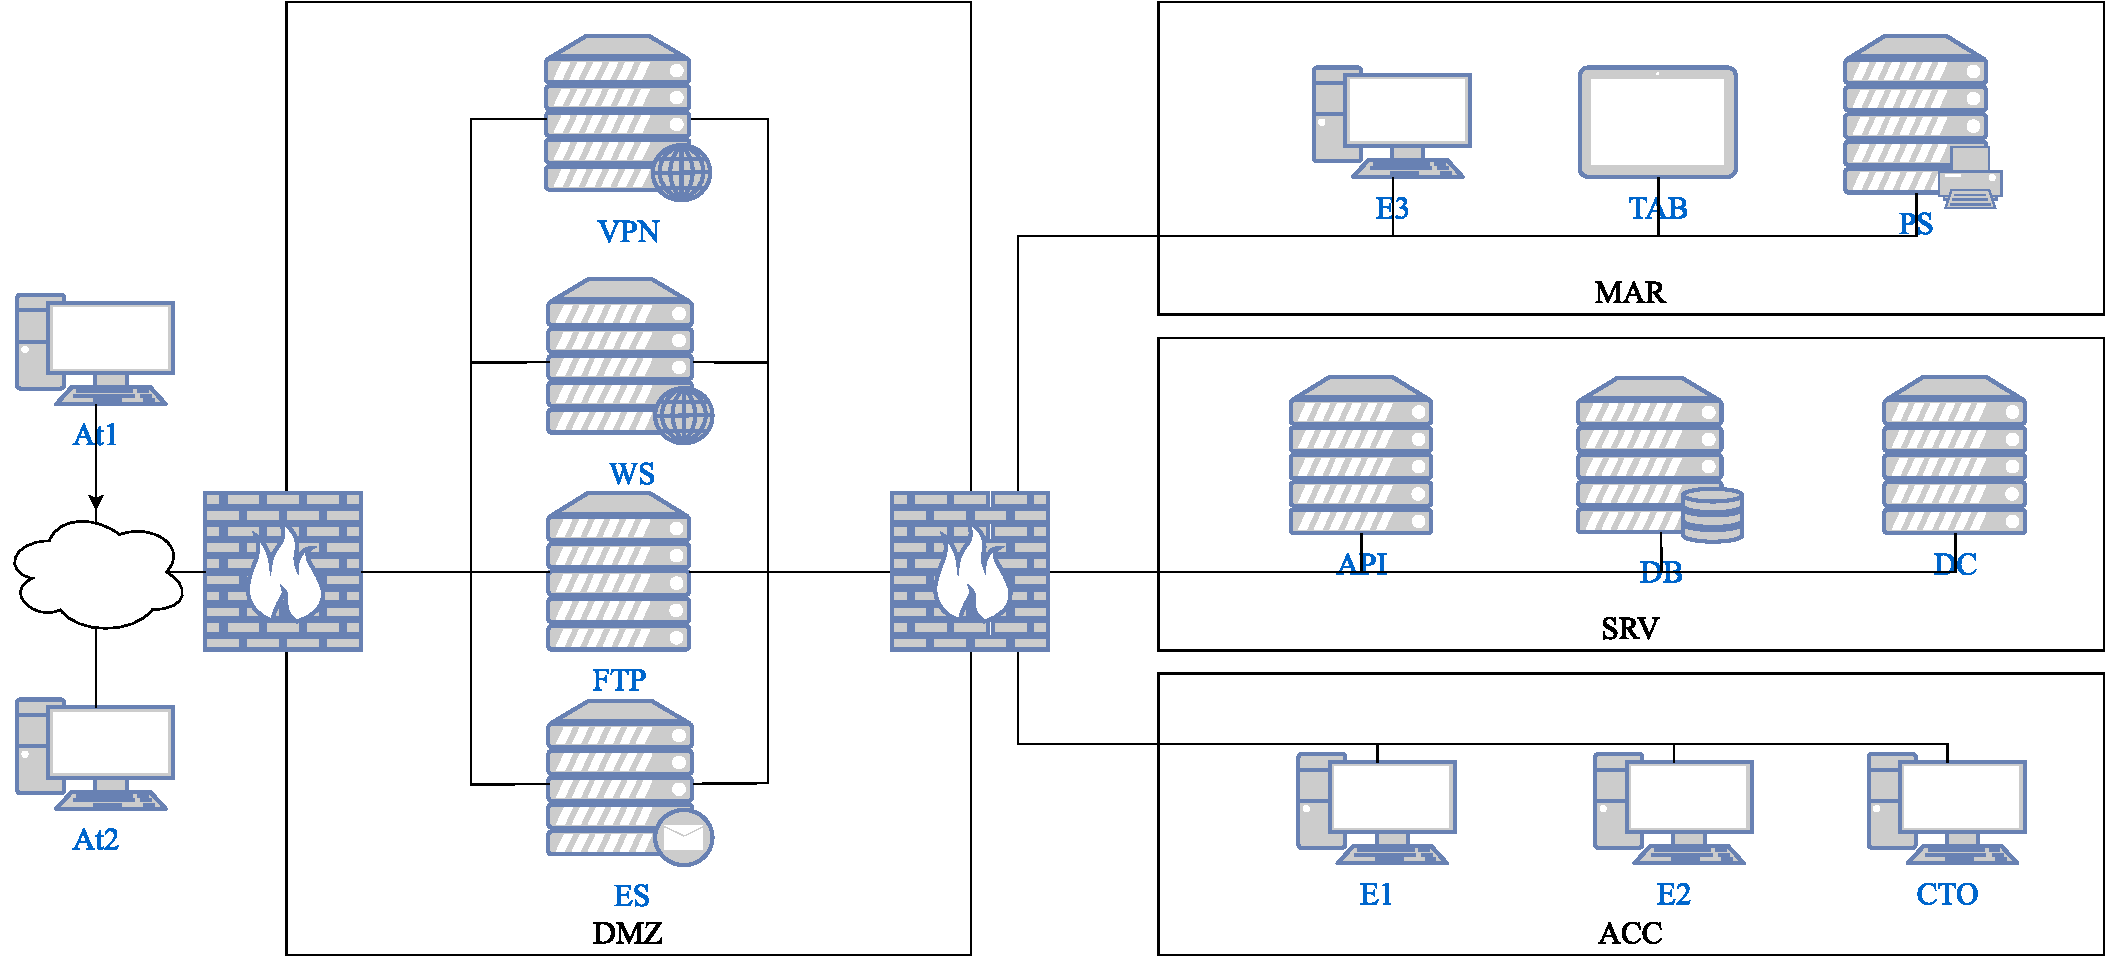
\includegraphics[width=\linewidth]{figures/topology.pdf}
  \caption{Topologie réseau proposée pour la simulation d’infrastructure d’entreprise}
  \label{fig:scenario_network_topology}
\end{figure}

L'arbre d'attaque-défense associé à ce scénario est illustré à la Figure~\ref{fig:ADTree}. Chaque nœud représente une étape clé dans la progression de l'attaque ou de la défense, avec des dépendances logiques entre les actions. Les agents rouges (attaquants) doivent enchaîner certaines actions pour atteindre leurs objectifs, tandis que les agents bleus (défenseurs) doivent anticiper et contrer ces mouvements. Cet arbre sert de base pour la modélisation des stratégies des agents dans l'environnement simulé.

\begin{figure}[h!]
  \centering
  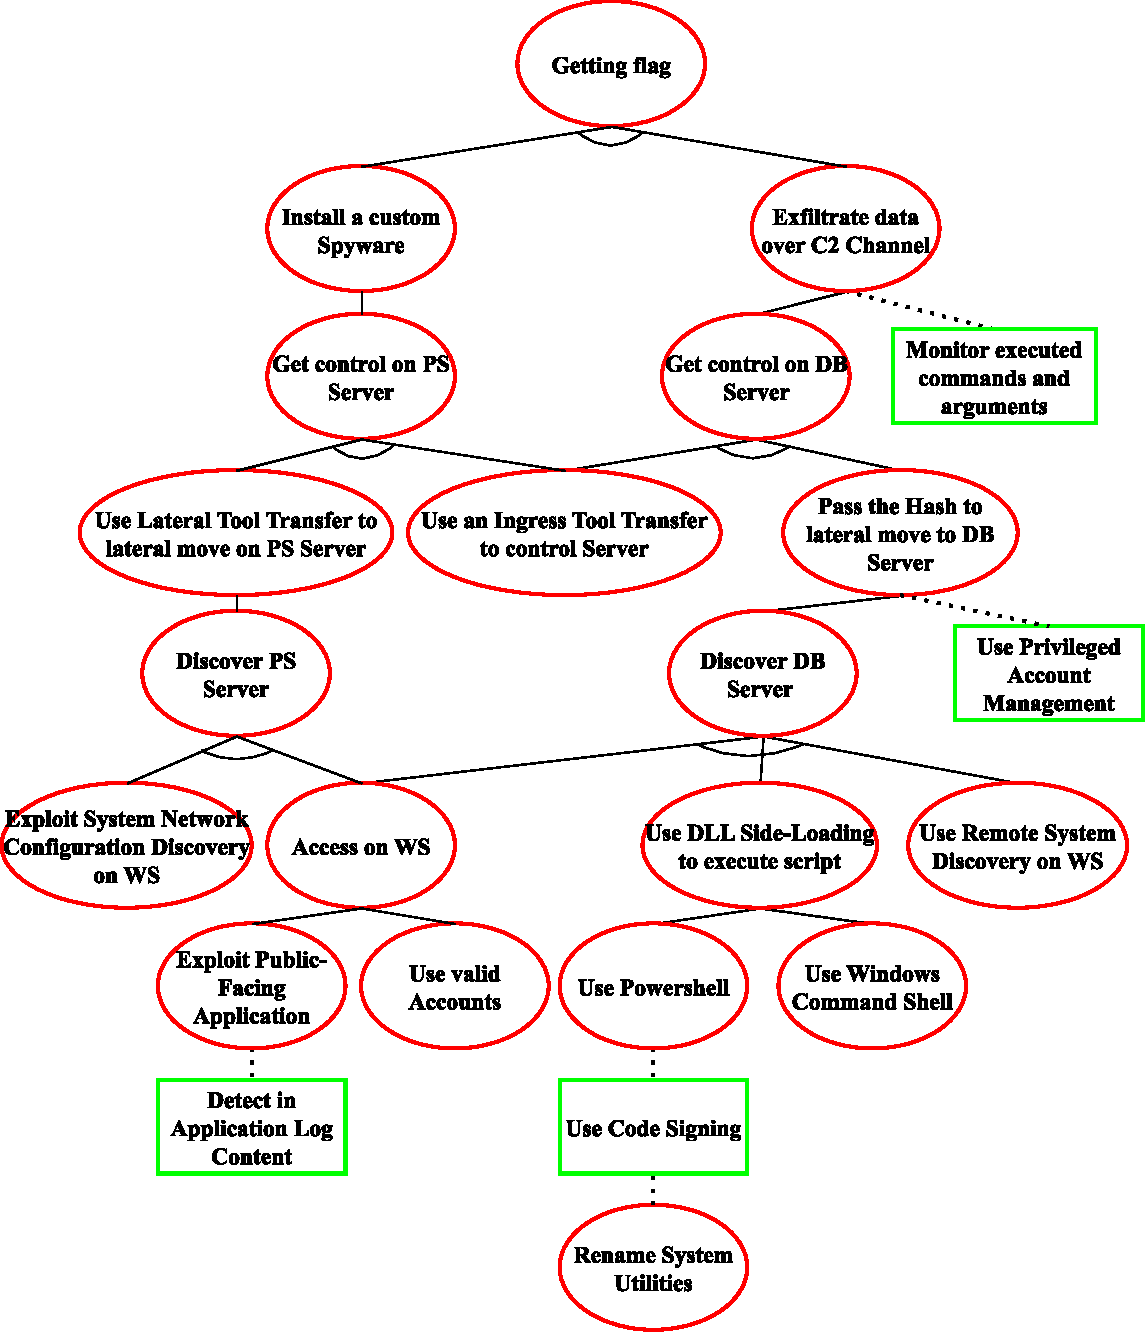
\includegraphics[width=0.8\linewidth]{figures/ADTree.pdf}
  \caption{Aperçu de l'arborescence AD proposée pour l'attaque/la défense}
  \label{fig:ADTree}
\end{figure}


\subsection{Spécificités par rapport au protocole générique}
\begin{itemize}
  \item \textbf{Modélisation (\acn{MOD-MAN})}~: environnement codé manuellement pour refléter les tactiques GALLIUM APT ; inclut services réseau, fichiers, et règles de sécurité.
  \item \textbf{Entraînement (\acn{TRN-UNC})}~: absence de guidage organisationnel pour servir de baseline ; sélection d’algorithmes orientés performance brute.
  \item \textbf{Analyse}~: centrée sur les métriques de performance et de scalabilité ; pas de calcul \acn{OF}/\acn{SOF}/\acn{FOF}.
  \item \textbf{Transfert}~: non appliqué, l’environnement simulé étant le contexte final.
\end{itemize}


\section{Essaim de drones}
\label{sec:drone_swarm}

Cette étude de cas évalue \acn{MAMAD} dans le scénario simulé du \textit{CAGE Challenge 3}~\cite{cage_challenge_3_announcement}, qui consiste à développer un SMA de cyberdéfense pour protéger un réseau ad hoc d’essaims de drones contre des attaques logicielles malveillantes.

\subsection{Instanciation du protocole}
\begin{table}[h!]
  \centering
  \caption{Instanciation du protocole pour le cas d’étude \emph{Essaim de drones}}
  \label{tab:proto_inst_drones}
  \renewcommand{\arraystretch}{1.2}
  {%

    \footnotesize

    \begin{tabular}{p{5cm}p{8.5cm}}
      \hline
      \textbf{Élément}                                  & \textbf{Valeur instanciée}                                                                                                                                                                                                                                                                                        \\
      \hline
      \textbf{Nom du scénario}                          & Cyberdéfense d’un essaim de drones (CAGE Challenge 3 – environnement CybORG).                                                                                                                                                                                                                                     \\

      \textbf{Activités / sous-activités MAMAD}         & \acn{MOD-MAN}, \acn{TRN-CON}, \acn{ANL-SMAN}.                                                                                                                                                                                                                                                                     \\

      \textbf{Objectifs expérimentaux spécifiques}      & (i) Évaluer l’efficacité du guidage organisationnel MOISE+MARL dans un environnement de cyberdéfense temps-réel ; (ii) Mesurer l’impact sur la convergence, la robustesse et la stabilité des politiques ; (iii) Comparer plusieurs modèles organisationnels (MASCARA–MOISE+, modèles manuels, sans contraintes). \\

      \textbf{Algorithmes MARL utilisés}                & \texttt{MAPPO} (version MARLlib, MLP 2 couches : 128/256 neurones, Adam LR=0,0003).                                                                                                                                                                                                                               \\

      \textbf{Spécifications organisationnelles}        & Modèles \textbf{Active Defense}, \textbf{Suspect Isolation}, \textbf{Manual}, \textbf{Free}. Chaque modèle définit rôles, missions et contraintes déontiques propres.                                                                                                                                             \\

      \textbf{Critères principaux ciblés}               & Performance globale, Cohérence organisationnelle, Robustesse, Scalabilité, Critères cyberdéfense spécifiques.                                                                                                                                                                                                     \\

      \textbf{Métriques associées}                      & Récompense moyenne, écart-type, temps de convergence, \acn{OF}, taux de respect des contraintes, \% moyen de drones infectés, \% moyen d’attaques réussies.                                                                                                                                                       \\

      \textbf{Baselines}                                & \textbf{Free} (aucune contrainte, MARL standard) ; \textbf{Manual} (organisation empirique sans MASCARA) ; modèles organisationnels MOISE+MARL pour comparaison.                                                                                                                                                  \\

      \textbf{Particularités de modélisation}           & \textbf{MOD-MAN} : adaptation manuelle de l’architecture MASCARA en spécifications MOISE+ adaptées au CAGE Challenge 3 ; création de rôles, missions et objectifs alignés sur les besoins du scénario.                                                                                                            \\

      \textbf{Hyperparamètres spécifiques}              & MAPPO configuré selon tests préliminaires MARLlib ; entraînement sur 70 itérations (128 épisodes/itération).                                                                                                                                                                                                      \\

      \textbf{Perturbations / conditions particulières} & Attaques logicielles dynamiques simulées par agents rouges ; transmissions légitimes simulées par agents verts.                                                                                                                                                                                                   \\

      \textbf{Nombre de runs}                           & 5 runs indépendants par condition.                                                                                                                                                                                                                                                                                \\

      \textbf{Seuils de validation}                     & Valeurs par défaut du protocole (\(\texttt{org\_fit}_{min}\), \(\overline{r}_{min}\), \(\sigma_{max}\)).                                                                                                                                                                                                          \\
      \hline
    \end{tabular}
  }
\end{table}

\subsection{Description du scénario}
Le scénario simule un conflit fictif dans lequel un réseau de drones autonomes (agents bleus) doit être protégé contre des attaques (agents rouges) tout en maintenant ses communications internes (agents verts).
Chaque catégorie d’agent dispose d’un ensemble d’actions spécialisées :
\begin{itemize}
  \item \textbf{Bleus (défense)}~: \textit{RetakeControl}, \textit{RemoveOtherSessions}, \textit{BlockTraffic}.
  \item \textbf{Rouges (attaque)}~: \textit{ExploitDroneVulnerability}, \textit{SeizeControl}, \textit{FloodBandwidth}.
  \item \textbf{Verts (transfert)}~: \textit{SendData}.
\end{itemize}
La récompense des bleus est calculée à partir du succès des communications, du contrôle des drones et de la sécurisation du réseau.

\subsection{Spécificités par rapport au protocole générique}
\begin{itemize}
  \item \textbf{Modélisation (\acn{MOD-MAN})}~: construction manuelle des modèles organisationnels en adaptant MASCARA à MOISE+.
  \item \textbf{Entraînement (\acn{TRN-CON})}~: utilisation du wrapper MAMAD pour appliquer les contraintes MOISE+MARL pendant l’apprentissage.
  \item \textbf{Analyse (\acn{ANL-SMAN})}~: application de TEMM avec affinage manuel pour vérifier cohérence et respect des contraintes.
  \item \textbf{Transfert}~: non appliqué dans ce scénario, l’évaluation se faisant intégralement en simulation.
\end{itemize}

\subsection{Critères et mesures spécifiques}
En plus des critères communs du protocole, les indicateurs spécifiques incluent :
\begin{itemize}
  \item Pourcentage moyen de drones infectés.
  \item Pourcentage moyen d’attaques réussies.
  \item Taux de respect des contraintes organisationnelles.
\end{itemize}

\section{Architecture de microservices}
\label{sec:microservices}

Cette étude de cas évalue \acn{MAMAD} dans un contexte d’auto-scaling de microservices Kubernetes soumis à des défaillances et conditions adverses (attaques DDoS, pannes de pods, contention de ressources), en utilisant le framework \textbf{KARMA} intégré dans \textbf{CybMASDE}.

\subsection{Instanciation du protocole}
\begin{table}[h!]
  \centering
  \caption{Instanciation du protocole pour le cas d’étude \emph{Architecture de microservices}}
  \label{tab:proto_inst_microservices}
  \renewcommand{\arraystretch}{1.2}
  {%

    \footnotesize

    \begin{tabular}{p{5cm}p{8.5cm}}
      \hline
      \textbf{Élément}                                  & \textbf{Valeur instanciée}                                                                                                                                                                                                                                    \\
      \hline
      \textbf{Nom du scénario}                          & Auto-scaling multi-agent pour la résilience opérationnelle dans un cluster Kubernetes « Services en chaîne » (CS).                                                                                                                                            \\

      \textbf{Activités / sous-activités MAMAD}         & \acn{MOD-AUT}, \acn{TRN-CON}, \acn{ANL-AUT}, \acn{TRF-AUT}.                                                                                                                                                                                                   \\

      \textbf{Objectifs expérimentaux spécifiques}      & (i) Évaluer la capacité de MAMAD à concevoir un HPA MAS optimisé pour différents types de défaillances ; (ii) Mesurer l’impact de contraintes organisationnelles sur la résilience opérationnelle ; (iii) Comparer avec systèmes HPA issus de la littérature. \\

      \textbf{Algorithmes MARL utilisés}                & \texttt{MAPPO} (MARLlib, MLP, 2 couches : 128/256 neurones, Adam LR=0,0003).                                                                                                                                                                                  \\

      \textbf{Spécifications organisationnelles}        & Quatre rôles alignés sur MOISE+ et AICA : Gestionnaire de goulots d’étranglement, Gestionnaire DDoS, Gestionnaire de pannes, Gestionnaire de ressources. Chaque rôle a une mission et un objectif basé sur des métriques.                                     \\

      \textbf{Critères principaux ciblés}               & Performance globale, Cohérence organisationnelle, Robustesse, Scalabilité, Qualité de la modélisation (jumeau numérique), Adaptabilité, Explicabilité.                                                                                                        \\

      \textbf{Métriques associées}                      & Récompense globale, taux de réussite (\%), ratio de requêtes en attente (\%), latence moyenne (ms), écart-type, précision du jumeau numérique (\%), temps de convergence, alignement comportement-rôle (\%).                                                  \\

      \textbf{Baselines}                                & HPA classiques : \textbf{AWARE}, \textbf{Gym-HPA}, \textbf{Rlad-core}. Études d’ablation : avec/sans MLP, avec/sans contraintes, multi-agent vs mono-agent.                                                                                                   \\

      \textbf{Particularités de modélisation}           & \acn{MOD-AUT} : génération automatique du jumeau numérique à partir de traces réelles du cluster et dérivation automatisée des rôles/missions.                                                                                                                \\

      \textbf{Hyperparamètres spécifiques}              & MAPPO configuré selon tuning MARLlib et contraintes de ressources Kubernetes ; scénarios simulés et mixtes.                                                                                                                                                   \\

      \textbf{Perturbations / conditions particulières} & Cinq scénarios : goulots d’étranglement, attaque DDoS, pannes de pod, contention des ressources, scénario mixte.                                                                                                                                              \\

      \textbf{Nombre de runs}                           & 5 runs indépendants par condition.                                                                                                                                                                                                                            \\

      \textbf{Seuils de validation}                     & Valeurs du protocole générique + seuils spécifiques à KARMA (\(Q_{\text{seuil}} = 30\), \(U_{\text{seuil}}=90\%\), etc.).                                                                                                                                     \\
      \hline
    \end{tabular}
  }
\end{table}

\subsection{Spécificités par rapport au protocole générique}
\begin{itemize}
  \item \textbf{Modélisation (\acn{MOD-AUT})}~: génération automatique d’un modèle Kubernetes via jumeau numérique, avec extraction automatique des spécifications organisationnelles.
  \item \textbf{Entraînement (\acn{TRN-CON})}~: intégration du wrapper MAMAD avec contraintes MOISE+MARL dans CybMASDE/KARMA.
  \item \textbf{Analyse (\acn{ANL-AUT})}~: utilisation automatisée de TEMM pour vérifier cohérence et alignement comportement-rôle.
  \item \textbf{Transfert (\acn{TRF-AUT})}~: déploiement direct des politiques entraînées dans un cluster Kubernetes réel via API.
\end{itemize}


\chapter{Résultats expérimentaux et analyse}

\section{Résultats et discussion des environnements non orientés Cyberdéfense}\label{sec:results_and_discussion_cyberdefense}

Cette section présente et analyse les résultats expérimentaux obtenus en appliquant MOISE+MARL dans différents environnements, en mettant en évidence les indicateurs clés et les comparaisons avec AGR+MARL.

\begin{table*}[h!]
  \centering
  \caption{Résultats détaillés pour chaque environnement et algorithme privilégié sous RB et OB.}
  \label{tab:detailed_results}
  \small
  \renewcommand{\arraystretch}{1.2}
  {%

    \footnotesize
    \begin{tabular}{p{3.5cm}p{1.5cm}p{1.cm}p{1.3cm}p{1cm}p{1.3cm}p{1.3cm}p{1.2cm}p{1.2cm}p{1cm}}
      \hline
      \textbf{Env.}               & \textbf{Alg.} & \textbf{Org. Spec.} & \textbf{Cum. Rew.} & \textbf{STD} & \textbf{Conv. Rate} & \textbf{Viol. Rate} & \textbf{Cons. Score} & \textbf{Score de vol} & \textbf{Niveau d'adéquation de l'organisation} \\ \hline
      Prédateur-proie             & MADDPG        &                     & 200,1              & 21,5         & 0,65                & 12,3\%              & -                    & 0,65                  & 0,43                                           \\
      Prédateur-Proie             & MADDPG        & Oui                 & 245,8              & 15,2         & 0,85                & 0,0\%               & 0,81                 & 0,83                  & 0,87                                           \\
      Overcooked-AI               & MAPPO         &                     & 348,2              & 15,6         & 0,75                & 7,1\%               & -                    & 0,71                  & 0,48                                           \\
      Overcooked-AI               & MAPPO         & Oui                 & 391,2              & 10,4         & 0,92                & 0,0\%               & 0,89                 & 0,89                  & 0,91                                           \\
      Gestion d'entrepôt          & Q-Mix         &                     & 257,4              & 18,9         & 0,74                & 7,8\%               & -                    & 0,68                  & 0,50                                           \\
      Gestion d'entrepôt et Q-Mix & Oui           & 307,1               & 13,8               & 0,88         & 0,0\%               & 0,88                & 0,86                 & 0,90                                                                   \\
      Cyberdéfense                & COMA          &                     & 162,4              & 17,3         & 0,70                & 12,2\%              & -                    & 0,67                  & 0,45                                           \\
      Cyberdéfense                & COMA          & Oui                 & 188,9              & 11,2         & 0,86                & 0,0\%               & 0,76                 & 0,80                  & 0,83                                           \\ \hline
    \end{tabular}
  }
\end{table*}

\subsection{Adéquation et cohérence organisationnelles quantitatives}

\autoref{tab:detailed_results} résume les mesures de performance pour chaque environnement et l'algorithme le plus efficace dans les deux cas, RB et OB. Dans tous les environnements, la mesure de l'adéquation organisationnelle est nettement plus élevée dans le cas OB, ce qui confirme que MOISE+MARL aligne efficacement les comportements des agents sur les spécifications organisationnelles.

Par exemple, dans l'environnement \textbf{Predator-Prey} avec \textbf{MADDPG}, les agents dans la configuration OB ont atteint un niveau d'adéquation organisationnelle de 0,87, ce qui représente une augmentation de 44 % par rapport au RB (0,43). De même, dans l'environnement \textbf{Overcooked-AI}, \textbf{MAPPO} sous OB a atteint une adéquation organisationnelle de 0,91 (soit une augmentation de 89 % par rapport à 0,48 sous RB). Ces améliorations se reflètent dans l'environnement \textbf{Warehouse Management} avec \textbf{Q-Mix}, où l'adéquation organisationnelle est passée de 0,50 dans le RB à 0,90 dans l'OB, ce qui suggère une efficacité constante de MOISE+MARL.

En général, les agents soumis à des contraintes organisationnelles présentent un écart de récompense plus faible et un taux de convergence plus élevé, ce qui suggère un impact sur leur comportement. Nous avons observé manuellement les interactions des agents dans des environnements visualisables tels que Predator-Prey et avons vérifié que les comportements des agents formés correspondent bien au comportement attendu d'une organisation implicite structurelle et fonctionnelle.
%
En effet, la variation significative en fonction de l'application des spécifications organisationnelles aux agents et l'alignement manuellement vérifié des agents avec leurs rôles suggèrent que le niveau d'adéquation organisationnelle est corrélé à l'adéquation organisationnelle.

Si l'on considère que le niveau d'adéquation organisationnelle est fiable dans tous les environnements, le \textbf{score de cohérence} affiche également des valeurs importantes, avec une valeur minimale de 0,76 pour l'environnement \textbf{Cyber-Defense}. Cela suggère que malgré un environnement bruyant qui introduit certaines perturbations dans le comportement des agents, les spécifications organisationnelles déduites restent proches de celles appliquées.

\subsection{Performances et stabilité des algorithmes}

Les résultats indiquent que les algorithmes basés sur des politiques et sur l'acteur-critique tels que \textbf{MADDPG} et \textbf{MAPPO} tirent largement parti du cadre MOISE+ MARL, notamment en termes de cohérence et de stabilité. Par exemple, \textbf{MAPPO} dans l'environnement \textbf{Overcooked-AI} a vu son écart type de récompense passer de 15,6 (RB) à 10,4 (OB), reflétant une politique plus stable avec moins de fluctuations comportementales. \textbf{MADDPG} dans \textbf{Predator-Prey} a également montré une tendance similaire, avec une baisse de l'écart type de 21,5 dans le RB à 15,2 dans l'OB, indiquant une fiabilité accrue.

En revanche, les algorithmes basés sur la valeur, tels que \textbf{Q-Mix}, ont maintenu des performances élevées en termes de récompense cumulative, mais ont affiché une plus grande variabilité en termes de cohérence. Par exemple, dans \textbf{Warehouse Management}, \textbf{Q-Mix} a atteint un écart type de récompense de 13,8 dans l'OB, une amélioration notable par rapport à 18,9 dans le RB, mais toujours supérieure à la stabilité observée dans les algorithmes basés sur des politiques. Cela suggère que si \textbf{Q-Mix} est efficace pour atteindre les objectifs des tâches, il peut nécessiter un ajustement supplémentaire pour les rôles avec MOISE+MARL afin d'améliorer la cohérence.

\subsection{Impact des contraintes organisationnelles sur la convergence des politiques, la robustesse et les taux de violation}

L'application de contraintes organisationnelles a entraîné des taux de convergence plus rapides dans tous les environnements. Dans l'environnement \textbf{Cyber-Defense}, \textbf{COMA} avec MOISE+MARL a convergé à un taux de 0,86, contre 0,70 dans le RB. Des tendances similaires ont été observées dans l'environnement \textbf{Gestion d'entrepôt} avec \textbf{Q-Mix}, qui a montré une amélioration de 0,74 dans le RB à 0,88 dans l'OB. Cette convergence accélérée peut être attribuée à l'orientation structurée des rôles et des missions, qui réduit l'espace de recherche des politiques.

Outre les résultats présentés où la dureté des contraintes est fixée à 1, nous avons observé que les taux de violation des contraintes étaient systématiquement plus élevés lorsque les contraintes organisationnelles étaient définies avec une dureté plus faible. Dans \textbf{Overcooked-AI}, \textbf{MAPPO} a enregistré un taux de violation nul avec une dureté des contraintes de 1, contre 7,1 % avec une dureté de 0. De même, dans \textbf{Warehouse Management}, \textbf{Q-Mix} a réduit le taux de violation de 7,8 % à zéro à mesure que la rigidité des contraintes augmentait. Cela confirme encore l'efficacité du cadre pour améliorer le respect des comportements souhaités.

De plus, nous avons observé une amélioration constante de la robustesse lorsque des spécifications organisationnelles ont été appliquées aux agents. Par exemple, \textbf{MADDPG} dans \textbf{Predator-Prey} et \textbf{MAPPO} dans \textbf{Overcooked-AI} ont obtenu des scores de cohérence élevés de 0,81 et 0,89, respectivement, indiquant que les agents ont suivi de près les rôles déduits. La robustesse s'est également améliorée, \textbf{MAPPO} dans \textbf{Overcooked-AI} obtenant un score de robustesse de 0,89, contre 0,71 dans le RB, ce qui souligne l'impact du cadre sur la résilience des agents face aux perturbations.

Cependant, on peut souligner un biais potentiel : les spécifications organisationnelles ont été spécialement conçues pour englober toutes les observations, en évitant les nouvelles situations non gérées.


\subsection{Comparaison entre MOISE+MARL et AGR+MARL}

\begin{table}[h!]
  \centering
  \caption{Comparaison des performances entre MOISE+MARL et AGR+MARL.}
  \label{tab:ablation_study}
  \small
  \renewcommand{\arraystretch}{1.1}
  {%

    \footnotesize

    \footnotesize

    \begin{tabular}{p{2cm}p{0.5cm}p{0.6cm}p{1.3cm}p{0.6cm}p{1.3cm}}
      \hline
      \textbf{Cadre} & \textbf{Env.} & \textbf{Taux de conversion} & \textbf{Score de robustesse} & \textbf{Adéquation organisationnelle} & \textbf{Récompense cumulative} \\ \hline
      MOISE+MARL     & PP            & 0,85                        & 0,83                         & 0,87                                  & 245,8                          \\
      AGR+MARL       & PP            & 0,75                        & 0,69                         & 0,56                                  & 208,4                          \\
      MOISE+MARL     & OA            & 0,92                        & 0,89                         & 0,91                                  & 391,2                          \\
      AGR+MARL       & OA            & 0,82                        & 0,75                         & 0,58                                  & 348,9                          \\
      MOISE+MARL     & WM            & 0,88                        & 0,86                         & 0,90                                  & 307,1                          \\
      AGR+MARL       & WM            & 0,76                        & 0,72                         & 0,61                                  & 278,6                          \\ \hline
    \end{tabular}
  }
\end{table}

\noindent \autoref{tab:ablation_study} met en évidence l'impact des objectifs intermédiaires dans MOISE+ MARL. Dans \textbf{Overcooked-AI}, \textbf{MAPPO} sous MOISE+MARL a obtenu une récompense cumulative de 391,2, avec une adéquation organisationnelle de 0,91, soit 33 % de plus que les 0,58 de AGR+MARL. De même, dans \textbf{Warehouse Management}, \textbf{Q-Mix} sous MOISE+MARL a obtenu une récompense cumulative de 307,1, soit une augmentation de près de 10 % par rapport aux 278,6 de AGR+MARL, avec un score de robustesse plus élevé (0,86 contre 0,72).

Dans l'ensemble, ces résultats soulignent l'importance des objectifs intermédiaires pour favoriser des comportements plus stables et axés sur les objectifs. En facilitant la voie vers l'objectif global, MOISE+MARL surpasse systématiquement AGR+MARL en termes de récompenses, de robustesse et d'adéquation organisationnelle dans les domaines Predator-Prey (PP), Warehouse Management (WM) et Overcooked-AI (OA).
Enfin, nous avons analysé l'impact de l'augmentation du nombre de contraintes organisationnelles sur la durée de la formation. Les résultats préliminaires suggèrent une croissance presque linéaire de la durée de la formation à mesure que le nombre de contraintes augmente~\footnotemark[2].

\section{Résultats et discussion du scénario d'infrastructure d'entreprise}\label{sec:results_and_discussion_infra}

\begin{figure}
  \centering
  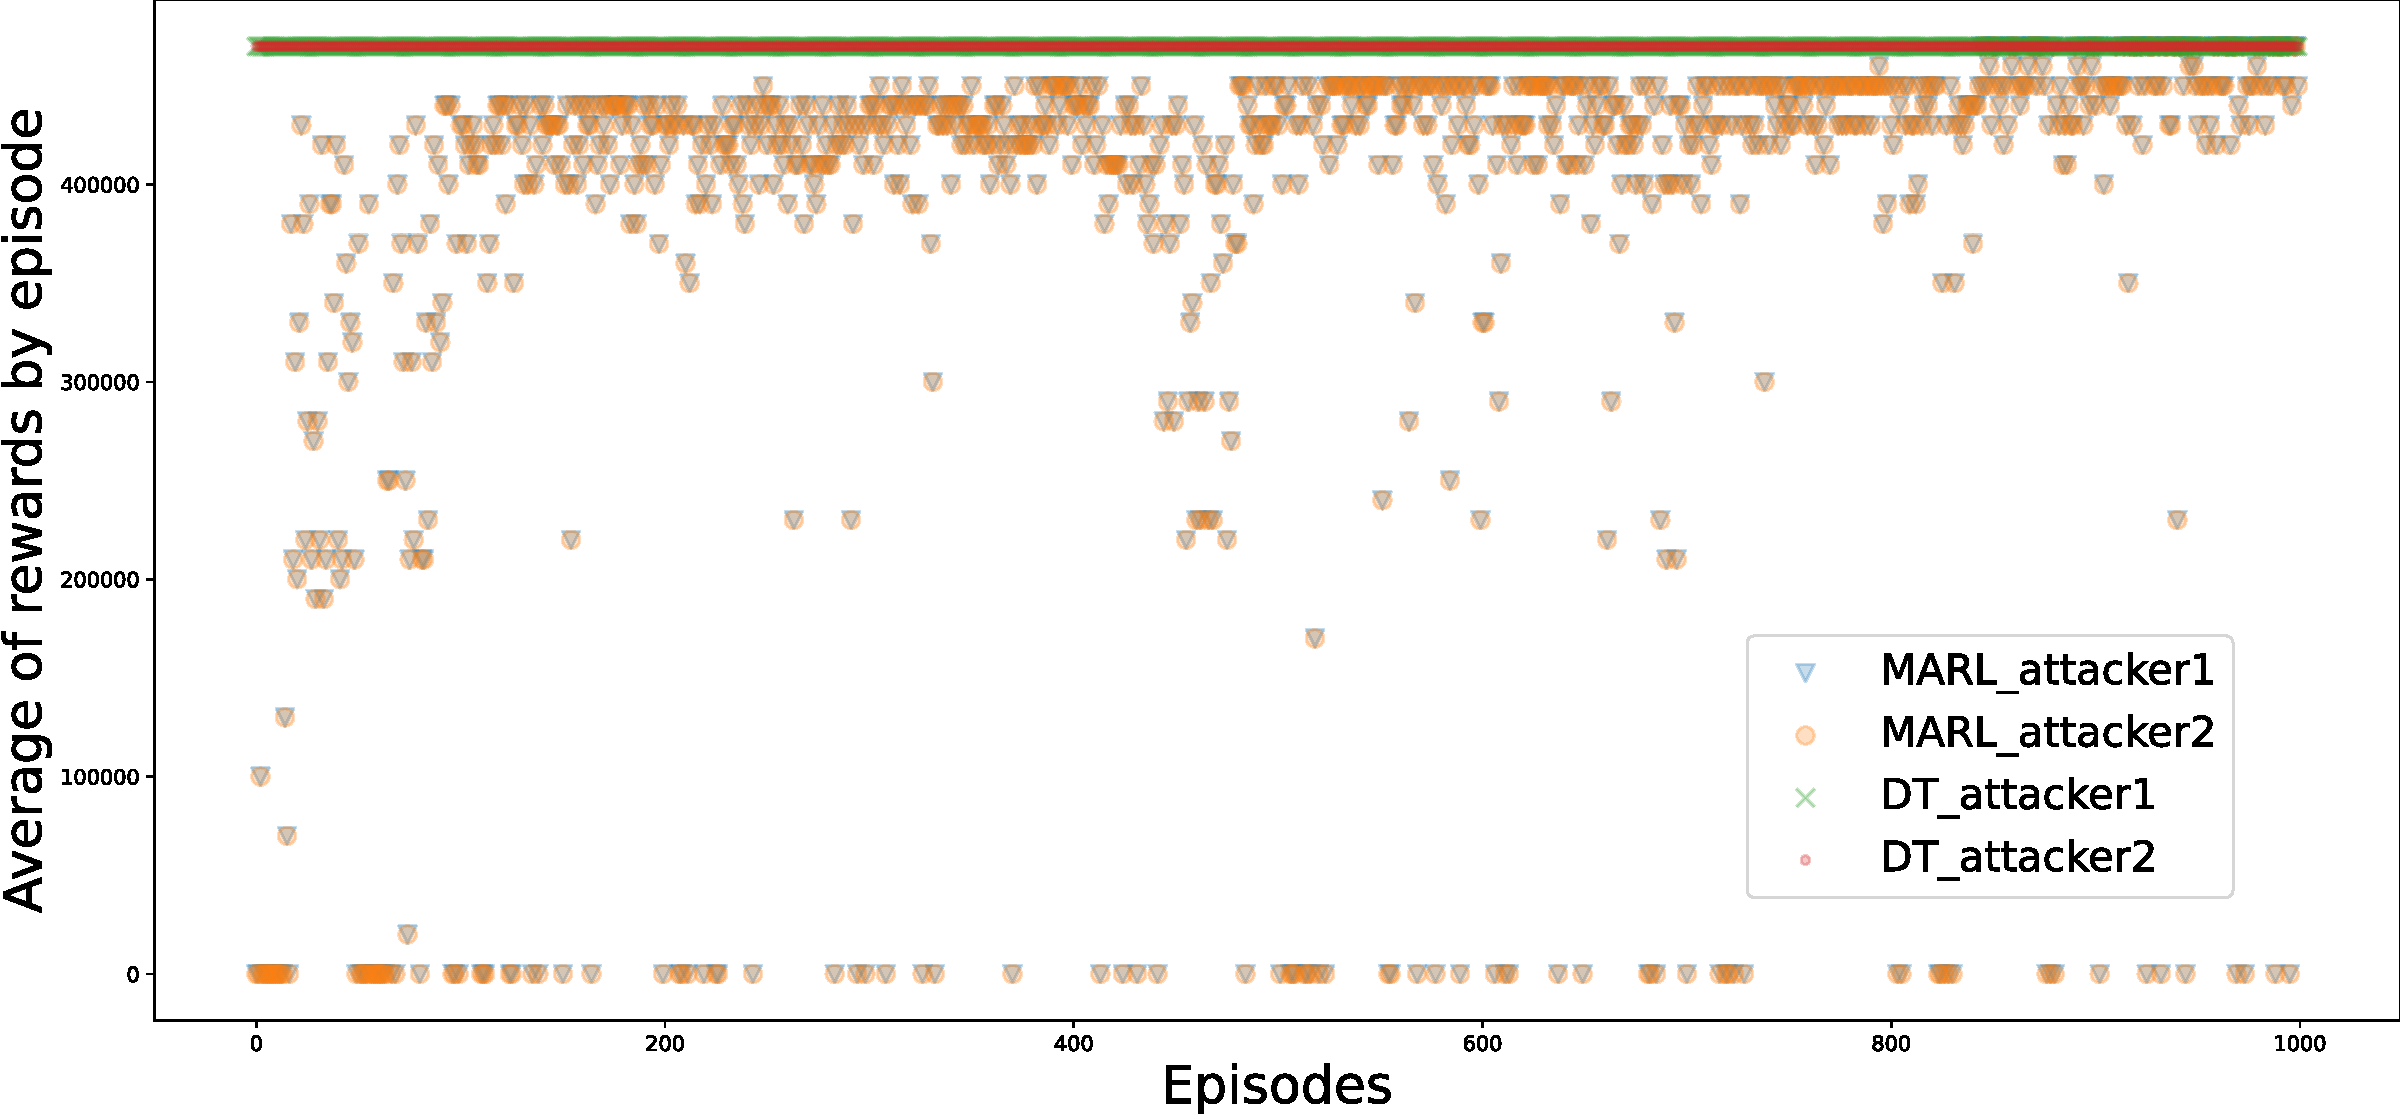
\includegraphics[width=\linewidth]{figures/graphs.pdf}
  \caption{Évolution de la moyenne des récompenses en fonction des épisodes dans des tests à petite échelle avec MARL et des approches par arbre de décision avec cyberdéfense inactive
  }
  \label{fig:graphs}
\end{figure}

\noindent
Les agents cyberattaquants sont initialement déployés sur At1 et At2, tandis que les agents cyberdéfenseurs sont déployés sur WS et DB. L'objectif ultime des attaquants est d'obtenir des données du serveur DB et d'installer un logiciel espion sur le serveur d'impression PS. Conformément à notre approche dans ~\ref{sec:ad_integration}, nous proposons une arborescence AD présentée dans la figure~\ref{fig:ADTree}. Elle montre uniquement les chemins que doivent suivre les attaques pour atteindre leur objectif final, tandis que les actions des défenseurs peuvent les empêcher à plusieurs étapes de l'attaque.
Nous nous sommes d'abord intéressés à la configuration des deux comportements des cyberattaquants, puis à ceux des deux cyberdéfenseurs. Nous avons simulé une version abstraite du scénario sur 1 000 épisodes.

% En outre, nous avons mis en œuvre d'autres actions courantes pour interagir avec le système de fichiers, la configuration du système d'exploitation, la configuration du pare-feu et les services réseau. Ces actions peuvent être dérivées des actions d'attaque/défense, mais ne sont pas implicitement représentées dans l'arbre AD. Elles sont toutefois prises en compte dans la simulation afin que les agents puissent explorer les chemins d'action, même si ceux-ci ne mènent pas à l'objectif final de l'attaquant.


%\subsection{Exécution et évaluation du scénario}

\noindent
\textbf{Approche aléatoire}~: \quad L'agent aléatoire choisit ses actions en explorant l'ensemble de l'espace d'action sans aucun critère jusqu'à ce qu'il atteigne l'objectif. Dans notre étude de cas, le chemin d'action le plus court permettant aux attaquants d'atteindre l'objectif final comprend 16 actions différentes parmi les 30 actions définies, ce qui correspond à une faible probabilité de $(1/30)^{16}$.
Cette approche permet d'obtenir un benchmark des cas de défaillance inattendus et de les comparer avec d'autres types d'agents.

\noindent
\textbf{Approche par arbre de décision (DT) }~: \quad L'arbre de décision a été appliqué afin d'obtenir une référence lorsque les cyberattaquants ou les cyberdéfenseurs connaissent déjà la meilleure action à entreprendre, le rôle de chaque agent étant défini par un DT.
Dans la figure~\ref{fig:graphs}, $DT\_attacker1$ suit un chemin d'action pour atteindre l'objectif d'installer un logiciel espion personnalisé dans PS. Dans le même temps, $DT\_attacker2$ atteint l'objectif d'exfiltrer des données dans DB et de terminer le chemin d'action en obtenant le drapeau. Nous avons ensuite ajouté les défenseurs $DT\_defender1$, qui doit détecter les journaux malveillants sur WS, et $DT\_defender2$, qui doit utiliser la gestion des comptes privilégiés ou surveiller les commandes et arguments exécutés sur DB. Nous avons observé que les attaquants étaient incapables d'atteindre leur objectif final.

\noindent
\textbf{Approche d'apprentissage par renforcement multi-agents (MARL)}~: \quad L'apprentissage Q~\cite{CWatkins1992} a été appliqué avec un apprentissage par programme afin que les attaquants apprennent d'abord comment atteindre l'objectif final de l'attaque avant d'ajouter des défenseurs.
Dans la figure~\ref{fig:graphs}, $MARL\_attacker1$ et $MARL\_attacker2$ suivent le même comportement, affinant finalement les actions appliquées pour atteindre l'objectif final. Après plusieurs épisodes, les chemins d'action choisis par les attaquants ont tendance à être aussi efficaces que les chemins DT. Lorsque nous avons ajouté les défenseurs $MARL\_defender1$ et $MARL\_defender2$, nous avons vérifié que les attaquants étaient de moins en moins capables d'atteindre l'objectif ultime.

\section{Résultats et discussion du scénario d'essaim de drones}\label{sec:results_and_discussion_essaim}

\autoref{fig:learning_curves} illustre les courbes d'apprentissage des modèles « Suspect Isolation », « Active Defensive » et « Manual », indiquant leurs taux de convergence au cours des épisodes d'entraînement.
\autoref{tab:metrics_comparison} résume le temps de convergence pendant l'entraînement ainsi que les récompenses moyennes, l'écart type, le nombre moyen de drones infectés et le nombre moyen d'attaques de logiciels malveillants obtenus par les modèles après une douzaine d'épisodes d'entraînement.

\begin{figure}[ht]
  \centering
  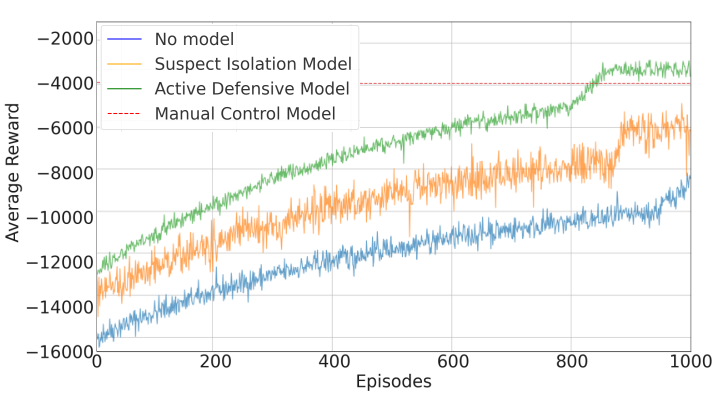
\includegraphics[width=1\linewidth]{figures/learning_curves.png}
  \caption{Courbes d'apprentissage pour \textit{Gratuit}, \textit{Isolation suspecte}, \textit{Défense active}, \textit{Manuel} en utilisant le mode \textit{correct\_policy} }
  \label{fig:learning_curves}
\end{figure}

\begin{table*}[t]
  \centering
  \setlength{\tabcolsep}{4.5pt}
  \caption{Comparaison des modèles et des modes de contrainte par rapport aux métriques.}
  \label{tab:metrics_comparison}
  {%

    \tiny

    \begin{tabular}{lcccccccccccc}
                                   & {Gratuit}   & \multicolumn{3}{c}{Isolation des suspects} & \multicolumn{3}{c}{Défense active} & {Manuel}                                                                                     \\
      % \cline{2-13}
      Métrique                     &             & Pénaliser                                  & Corriger                           & Corriger\_Politique & Pénaliser & Corriger & Corriger\_Politique &                           \\
      \midrule
      Récompense moyenne           & -8727,49    & -5900,00                                   & -6085,12                           & -6088,00            & -3055,36  & -3100,00 & -3060,00            & -3906,00                  \\
      Écart type                   & 138,00      & 2148,0                                     & 2027,0                             & 2018,00             & 962,      & 940,00   & 945,00              & 570,33                    \\
      Évolutivité                  & Moyenne     & Élevée                                     & Moyenne                            & Moyenne             & Élevée    & Moyenne  & Moyenne             & Moyenne                   \\
      Temps de convergence         &             & gt;1000                                    & 1000                               & 950                 & 950       & 800      & 850                 & 850         & $\emptyset$ \\
      Respect des contraintes      & $\emptyset$ & Faible                                     & Élevé                              & Élevé               & Moyen     & Élevé    & Élevé               & $\emptyset$               \\
      Moyenne inf. drones (\%)     & 61,0        & 43,0                                       & 30,0                               & 23,0                & 24,0      & 25,0     & 20,0                & 40,0                      \\
      Moyenne attaque malware (\%) & 72,0        & 55,0                                       & 52,0                               & 45,0                & 38,0      & 45,0     & 40,0                & 51,0                      \\
    \end{tabular}
  }
\end{table*}

Les modèles organisationnels ont efficacement influencé le comportement des drones dans l'environnement CybORG CAGE Challenge 3. Le modèle « Suspect Isolation » (isolement des suspects) a démontré son efficacité dans l'identification et l'isolement des drones présentant des activités suspectes, renforçant ainsi la sécurité globale. Ce modèle a permis d'identifier et de neutraliser rapidement les menaces potentielles, empêchant ainsi la propagation d'activités malveillantes au sein du essaim de drones ($\mathbf{C_1}$).

\autoref{fig:learning_curves} fournit une vue d'ensemble des courbes d'apprentissage pour chaque modèle. Le modèle « Free » (bleu) a présenté la convergence la plus lente et les récompenses moyennes les plus faibles. De plus, il montre également une faible variabilité des récompenses, ce qui indique que les agents sont lentement formés avec des changements limités à chaque étape. Ce résultat est prévisible, car le taux d'apprentissage pour MAPPO est relativement faible.

En revanche, le modèle « Suspect Isolation » (orange) a montré une convergence plus rapide et des récompenses moyennes plus élevées que le modèle « Free ». Cependant, la variabilité accrue (par rapport au modèle « Free ») suggère que, comme les agents sont contraints/incités à respecter certaines règles pour identifier et isoler les activités suspectes, leurs politiques peuvent nécessiter un certain temps pour s'habituer à ces règles et atteindre un comportement plus stable.

Le modèle « Active Defense » (vert) a affiché les récompenses moyennes les plus élevées et la convergence la plus rapide parmi tous les modèles. L'augmentation constante des récompenses démontre l'efficacité des stratégies de défense proactive mises en œuvre par les agents. Ce modèle a montré la plus grande amélioration des performances, soulignant les avantages de l'utilisation de contraintes organisationnelles structurées pour guider le comportement des agents. Le modèle « Active Defense » présente également une variabilité des récompenses plus faible que le modèle « Suspect Isolation », mais plus élevée que le modèle « Free ». Cela suggère que, même si les agents sont encore en activité d'adaptation aux contraintes, leurs comportements possibles sont plus limités dans le modèle « Active Defense » que dans le modèle « Suspect Isolation ».

Le modèle « Manuel » (ligne rouge en pointillés) a servi de référence pour la comparaison. Il a obtenu de meilleurs résultats que les modèles « Libre » et « Isolation des suspects », mais a été surpassé par le modèle « Défense active ». Cela s'explique par le fait que la stratégie de contrôle manuel, bien qu'efficace, manquait de l'adaptabilité et de l'efficacité fournies par les modèles organisationnels appris.

D'un point de vue quantitatif, les mesures fournissent également des preuves des avantages liés à l'application de contraintes organisationnelles. Comme l'illustre la figure \autoref{fig:learning_curves}, dans le cas d'une politique contrainte, les agents ont convergé plus rapidement que dans le modèle « Libre » dans tous les modes. Cela confirme que les contraintes organisationnelles peuvent accélérer l'apprentissage ($\mathbf{C_2}$). Comme prévu, la politique élaborée manuellement a permis une convergence immédiate, en raison de l'absence d'apprentissage.

Les mesures de récompense moyenne révèlent que les agents guidés par le modèle « Suspect Isolation » ont systématiquement surpassé ceux du modèle « Free », obtenant des récompenses plus élevées ($\mathbf{C_3}$). Cela indique que les contraintes organisationnelles améliorent non seulement l'efficacité de l'apprentissage, mais aussi les performances globales. Les politiques élaborées manuellement ont systématiquement obtenu les récompenses les plus élevées, soulignant l'efficacité de contraintes bien définies.

En ce qui concerne les modèles contraints, l'écart type dans \autoref{tab:metrics_comparison} a diminué progressivement du modèle le moins contraint, tel que « Suspect Isolation », au modèle le plus contraint, tel que « Active Defense » ($\mathbf{C_4}$). Cette réduction de la variabilité suggère que les contraintes organisationnelles contribuent à un comportement plus stable et plus cohérent des agents.

Le critère de respect des contraintes a été pleinement satisfait dans les modes \textit{correct} et \textit{correct\_policy}, mais pas dans le mode \textit{penalize} ($\mathbf{C_5}$). Cela démontre que si les agents peuvent apprendre à respecter efficacement les contraintes, le mode d'intégration des contraintes joue un rôle crucial. Dans notre évaluation, les modes « correct » et « correct\_policy » ont démontré une adhésion totale aux contraintes organisationnelles, comme en témoigne l'absence totale de déviations dans le comportement des agents par rapport aux rôles et missions prescrits. En revanche, le mode « pénaliser » a montré des déviations occasionnelles, en particulier dans les modèles peu contraints tels que « Suspect Isolation ». Cela suggère que les agents privilégient parfois la maximisation des récompenses plutôt que le respect strict des contraintes. Une analyse plus approfondie des stratégies de pénalisation permettrait d'améliorer la conformité.

L'évolutivité, évaluée en analysant les performances du système lorsque le nombre d'agents et d'obstacles augmente, a été gérée efficacement dans tous les modèles ($\mathbf{C_6}$). En particulier, le mode \textit{penalize} a montré une évolutivité supérieure grâce à un calcul efficace intégré des mises à jour des politiques, contrairement aux modes \textit{correct} et \textit{correct\_policy} qui nécessitent des fonctions de correction supplémentaires.

Les modèles « Active Defense » et « Suspect Isolation » ont tous deux eu un impact sur les indicateurs « Pourcentage moyen de drones infectés » et « Pourcentage moyen d'attaques de logiciels malveillants réussies » ($\mathbf{C_7}$ et $\mathbf{C_8}$). Cependant, il est important de noter que ces deux indicateurs ne sont pas directement liés à la récompense globale, car ils sont calculés séparément. Le modèle « Active Defense » a obtenu les meilleurs résultats, réduisant le pourcentage de drones infectés à 23 % et le taux de réussite des attaques de logiciels malveillants à 38 %. Cette réduction significative, comparée au taux d'infection de 61 % et au taux de réussite de 72 % du modèle « Free », démontre l'efficacité des stratégies défensives proactives dans la prévention de la propagation des logiciels malveillants et des attaques réussies. Le modèle « Isolation des suspects » a également affiché des taux d'infection et de réussite des attaques inférieurs à ceux du modèle « Libre ».

% Ces résultats soulignent l'importance de mettre en œuvre des contraintes organisationnelles structurées et des mécanismes de défense proactifs au sein des systèmes autonomes. L'intégration des modèles organisationnels $\mathcal{M}OISE^+$ dans le cadre MARL, comme le démontre MAMAD, améliore considérablement l'efficacité et la coordination des agents de cyberdéfense autonomes. Les résultats expérimentaux soulignent que les contraintes organisationnelles structurées améliorent non seulement les performances et la stabilité des agents, mais garantissent également que leur comportement est conforme aux objectifs de la mission et aux objectifs de cybersécurité.

% Les résultats suggèrent qu'un affinement des spécifications organisationnelles et l'intégration de règles et de protocoles plus sophistiqués pourraient améliorer encore davantage le comportement et la coordination des agents. Ce développement continu promet de renforcer la résilience et la robustesse des stratégies de cyberdéfense face à des menaces de plus en plus sophistiquées.
% Cependant, la généralisation de MAMAD à différents scénarios de cyberdéfense réels, tels que la sécurité de l'IoT ou les systèmes de contrôle industriel, pourrait nécessiter des ajustements des spécifications organisationnelles et des contraintes politiques. Les travaux futurs devraient explorer ces adaptations afin de valider la large applicabilité de MAMAD.

\section{Résultats et discussion du scénario d'architecture de microservices}\label{sec:results_and_discussion_ms}

Cette section analyse les performances de KARMA dans la résolution des six lacunes identifiées pour le scénario de l'architecture de microservices.

\subsection{Lacune 1 : Résilience opérationnelle}
La résilience opérationnelle évalue la capacité du système à gérer les défaillances et à maintenir une qualité de service élevée.
\begin{table}[h]
  \centering
  \caption{Indicateurs de résilience opérationnelle dans tous les scénarios.}
  \label{tab:operational_resilience}

  {\footnotesize
    \begin{tabular}{>{\raggedright\arraybackslash}m{2.7cm}>{\centering\arraybackslash}m{1.5cm}>{\centering\arraybackslash}m{1.5cm}>{\centering\arraybackslash}m{1.5cm}}
      \hline
      \textbf{Référence}                                                           & \textbf{Taux de réussite (\%)} & \textbf{Conformité en matière de latence (\%)} & \textbf{Demandes en attente (\%)} \\
      \hline
      KHPA                                                                         & 64,8                           & 58,1                                           & 20,7                              \\
      Gym-HPA                                                                      & 73,1                           & 65,7                                           & 20,8                              \\
      Rlad-core                                                                    & 77,4                           & 70,1                                           & 15,9                              \\
      AWARE                                                                        & 80,6                           & 73,8                                           & 13,3                              \\
      Agent unique sans spécificité organique                                      & 72,6                           & 65,4                                           & 17,0                              \\
      Agent unique avec spécification organisationnelle stricte                    & 80,8                           & 72,5                                           & 15,4                              \\
      Multi-agent sans spécification organisationnelle                             & 87,7                           & 81,5                                           & 9,3                               \\
      Multi-agent avec spécifications organisationnelles souples                   & 82,0                           & 74,7                                           & 15,0                              \\
      \textbf{Multi-agents avec spécifications organisationnelles rigides (KARMA)} & \textbf{90,9}                  & \textbf{85,7}                                  & \textbf{5,9}                      \\
      \hline
    \end{tabular}}
\end{table}
%
\autoref{tab:operational_resilience} présente une comparaison entre KARMA et les références existantes. Les résultats montrent que KARMA atteint le taux de réussite le plus élevé (\textbf{90,9\%}), surpassant toutes les références, y compris AWARE (80,6\%) et Rlad-core (\textbf{77,4\%}). De même, la conformité de KARMA en matière de latence est la plus élevée avec \textbf{85,7\%}, tandis que le taux de requêtes en attente le plus bas (\textbf{5,9\%}) suggère une gestion efficace des variations de charge de travail.

\noindent \textit{Remarque statistique :} Toutes les valeurs indiquées représentent la moyenne de 10 évaluations indépendantes. Bien que cela ne soit pas indiqué dans les tableaux par souci de concision, l'écart type entre les évaluations est resté faible ($\pm$1,8\% pour le taux de réussite et $\pm$2,1 ms pour la latence dans le scénario mixte), ce qui indique des résultats robustes.

Les performances de KARMA découlent de sa coordination multi-agents structurée, qui répartit de manière optimale les ressources en fonction des contextes de défaillance, évitant ainsi les actions de mise à l'échelle redondantes ou conflictuelles, problèmes courants dans les autoscalers basés sur le RL à agent unique.
%
Les autoscalers réactifs basés sur des seuils, tels que KHPA et Gym-HPA, ont du mal à gérer les charges de travail dynamiques, ce qui entraîne une augmentation des demandes en attente et une baisse des taux de réussite. AWARE et Rlad-core améliorent le temps de réponse et le débit, mais ne disposent pas d'une coordination multi-agents, ce qui se traduit par des réactions plus lentes dans les scénarios adversaires. Les systèmes à agent unique sans spécifications organisationnelles souffrent d'une allocation inefficace des ressources, tandis que les systèmes à agent unique avec spécifications organisationnelles rigides bénéficient d'une prise de décision structurée, mais manquent encore de coordination distribuée.

La coordination basée sur les rôles de KARMA minimise les inefficacités et améliore la stabilité des décisions. Sa décomposition hiérarchique des objectifs permet des décisions indépendantes mais complémentaires, ce qui se traduit par une mise à l'échelle automatique plus résiliente.

Les résultats soulignent également la valeur des contraintes organisationnelles. Les systèmes multi-agents avec des contraintes souples (taux de réussite de 82,0 %) surpassent les approches à agent unique, mais les contraintes strictes de KARMA obtiennent les meilleurs résultats, éliminant les comportements conflictuels des agents et optimisant la mise à l'échelle.



\subsection{Écart 2 : Conditions adverses}

Les conditions adverses évaluent la robustesse du système face à des scénarios perturbateurs tels que les attaques DDoS.
\begin{table}[h]
  \centering
  \caption{Performances dans un scénario DDoS.}
  \label{tab:adversarial_conditions}


  {
    \footnotesize
    \begin{tabular}{>{\raggedright\arraybackslash}m{3.6cm}>{\centering\arraybackslash}m{1.8cm}>{\centering\arraybackslash}m{2cm}}
      \hline
      \textbf{Référence}                                                           & \textbf{Temps de récupération (s)} & \textbf{Disponibilité du service (\%)} \\
      \hline
      KHPA                                                                         & 80,7                               & 65,6                                   \\
      Gym-HPA                                                                      & 66,2                               & 72,6                                   \\
      Rlad-core                                                                    & 37,4                               & 78,3                                   \\
      AWARE                                                                        & 49,5                               & 83,6                                   \\
      Agent unique sans spécificité organique                                      & 60,3                               & 72,4                                   \\
      Agent unique avec spécificité organisationnelle dure                         & 48,5                               & 77,5                                   \\
      Multi-agent sans spécification organisationnelle                             & 43,5                               & 82,0                                   \\
      Multi-agent avec spécifications organisationnelles souples                   & 38,8                               & 86,0                                   \\
      \textbf{Multi-agent avec spécifications organisationnelles strictes (KARMA)} & \textbf{33,0}                      & \textbf{90,7}                          \\
      \hline
    \end{tabular}}
\end{table}
%
\autoref{tab:adversarial_conditions} compare les temps de récupération et la disponibilité du service dans le scénario \textit{Attaque DDoS}. KARMA atteint le temps de récupération le plus rapide (\textbf{33,0 s}), surpassant AWARE (\textbf{38,8 s}) et Rlad-core (\textbf{43,5 s}). Il garantit également une bonne disponibilité du service à \textbf{90,7\%}, réduisant ainsi les temps d'indisponibilité par rapport à AWARE (\textbf{83,6\%}).

Les autoscalers traditionnels tels que KHPA et Gym-HPA s'appuient sur une mise à l'échelle réactive basée sur des seuils, ce qui entraîne une récupération plus lente et une disponibilité du service plus faible en cas d'attaques. Les méthodes basées sur le RL telles que Rlad-core et AWARE améliorent la résilience, mais manquent de coordination structurée, ce qui les rend moins efficaces contre les pics adverses. Les approches à agent unique ont du mal à trouver un équilibre entre l'atténuation des attaques et l'optimisation des ressources, tandis que les modèles multi-agents avec des contraintes souples permettent des actions exploratoires qui retardent parfois les réponses optimales.

L'apprentissage proactif et la coordination structurée de KARMA lui permettent d'anticiper les attaques plutôt que de réagir après une dégradation. Des contraintes explicites basées sur les rôles garantissent que les agents donnent la priorité aux actions de mise à l'échelle critiques, ce qui se traduit par une atténuation plus rapide et une disponibilité plus élevée. Ces résultats soulignent l'efficacité de l'apprentissage structuré multi-agents dans la mise à l'échelle automatique sensible à la sécurité, où les méthodes traditionnelles présentent une adaptation plus lente et des temps d'arrêt prolongés.


\subsection{Lacune 3 : Modélisation des jumeaux numériques}

\begin{table}[h]
  \centering
  \caption{Précision des modèles de transition dans tous les scénarios.}
  \label{tab:digital_twin_accuracy}

  {
    \footnotesize
    \begin{tabular}{>{\raggedright\arraybackslash}m{6cm}>{\centering\arraybackslash}m{2cm}}
      \hline
      \textbf{Référence}                             & \textbf{Précision (\%)} \\
      \hline
      Sans modèle de transition MLP                  & 83,5                    \\
      \textbf{Avec modèle de transition MLP (KARMA)} & \textbf{94,9}           \\
      \hline
    \end{tabular}}
\end{table}
%
La précision du modèle de jumeau numérique est essentielle pour former des agents dans des conditions réalistes.
\autoref{tab:digital_twin_accuracy} compare la précision de différents modèles de jumeaux numériques. Les résultats montrent que KARMA atteint une précision de \textbf{94,9\%}, surpassant le modèle non MLP (\textbf{83,5\%}), qui peine à généraliser.

Cette amélioration découle de la capacité du modèle MLP à saisir les dépendances non linéaires entre les fluctuations de la charge de travail, l'allocation des ressources et les actions de mise à l'échelle. Sans cette fonctionnalité, le système ne parvient pas à modéliser avec précision les comportements complexes des clusters.
%
En exploitant un réseau neuronal pour la modélisation des transitions, KARMA garantit un jumeau numérique plus fiable, permettant aux agents de s'entraîner dans des conditions proches de la réalité. Cela réduit le risque de mauvaises décisions lors du transfert des politiques vers la production, renforçant ainsi l'importance des simulations haute fidélité.



\subsection{Lacune 4 : Génération automatisée de SMA}

L'efficacité de la génération d'un SMA est évaluée en termes de temps de convergence et de surcoût de formation. \autoref{tab:mas_generation_efficiency} présente les résultats pour les différents scénarios concernés, tandis que \autoref{fig:learning_curves} montre les courbes d'apprentissage dans le scénario mixte sur 2000 épisodes.

\begin{table}[h!]
  \centering
  \caption{Efficacité de la génération de SMA dans tous les scénarios.}
  \label{tab:mas_generation_efficiency}
  {
    \footnotesize
    \begin{tabular}{>{\raggedright\arraybackslash}m{3.5cm}>{\centering\arraybackslash}m{2cm}>{\centering\arraybackslash}m{2cm}}
      \hline
      \textbf{Référence}                                                            & \textbf{Temps de convergence (épisodes)} & \textbf{Charge de formation (heures)} \\
      \hline
      Multi-agents sans spécifications organisationnelles                           & 1800                                     & 4                                     \\
      \textbf{Multi-agents avec spécifications organisationnelles strictes (KARMA)} & \textbf{950}                             & \textbf{1,5}                          \\
      \hline
    \end{tabular}}
\end{table}

L'apprentissage guidé par les rôles réduit l'espace de recherche des politiques optimales, ce qui permet une convergence plus rapide et une réduction des coûts de calcul. Ces gains d'efficacité sont particulièrement importants pour adapter les solutions SMA à des environnements complexes.

Les courbes d'apprentissage dans \autoref{fig:learning_curves} montrent que KARMA atteint une convergence stable beaucoup plus rapidement que la référence sans spécifications organisationnelles. À l'épisode 950, KARMA présente une variance minimale dans les récompenses cumulées, tandis que la référence nécessite près du double d'épisodes (1800) pour atteindre des performances comparables. Cela souligne le rôle des contraintes organisationnelles dans l'orientation des agents vers des politiques efficaces, réduisant ainsi les coûts d'exploration.

\noindent \textit{Discussion sur la charge :} La activité d'entraînement de KARMA a nécessité environ 1,5 heure sur une machine haute performance équipée d'un GPU (Tesla V100, 16 Go) et de 16 cœurs CPU, avec une convergence en moins de 1 000 épisodes. Au moment de l'inférence, la politique de chaque agent produit des décisions en moins de 30 ms, avec une empreinte mémoire négligeable (moins de 50 Mo par agent).

\autoref{tab:mas_generation_efficiency} montre une réduction du \textit{temps de convergence} d'environ \textbf{47\%} par rapport à Multi-Agent w/o Org. Spec., démontrant l'efficacité de l'apprentissage guidé par les rôles pour minimiser les explorations inutiles. De plus, la \textit{surcharge de formation} est réduite de \textbf{62,5\%}, ce qui démontre une meilleure praticité pour les systèmes à grande échelle où les ressources informatiques constituent un facteur limitant.

\begin{figure}[h!]
  \centering
  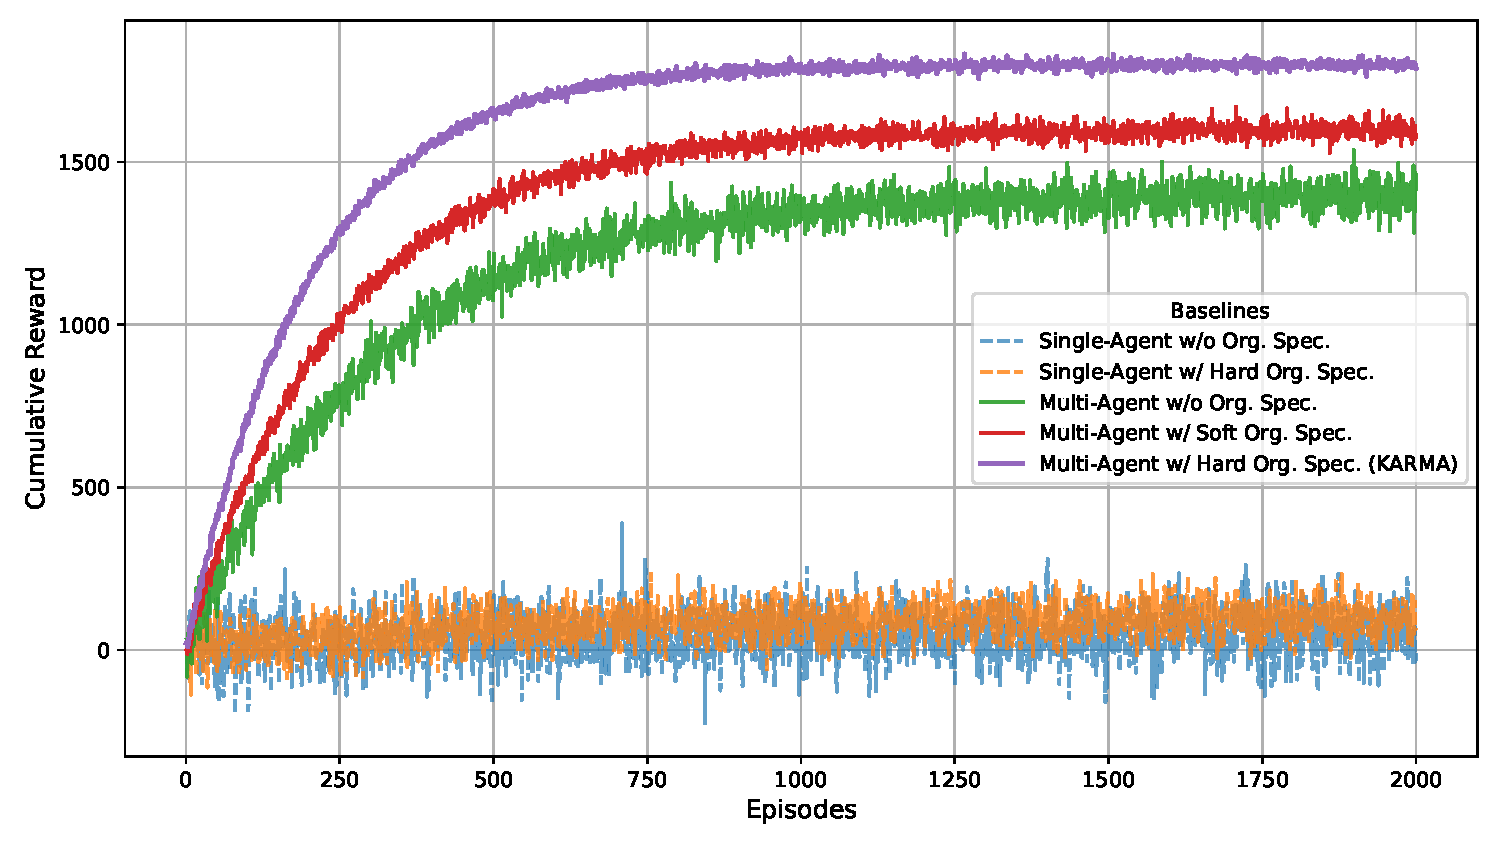
\includegraphics[width=0.49\textwidth]{figures/learning_curves.pdf}
  \caption{Courbes d'apprentissage entre les lignes de base pour le scénario mixte sur 2000 épisodes.}
  \label{fig:learning_curves}
\end{figure}


\subsection{Écart 5 : Adaptabilité}

L'adaptabilité évalue la capacité du système à maintenir ses performances sous des charges de travail dynamiques dans différents scénarios.
\begin{table}[h]
  \centering
  \caption{Comparaison de l'adaptabilité dans le scénario mixte.}
  \label{tab:adaptability_comparison}
  {
    \footnotesize
    \begin{tabular}{>{\raggedright\arraybackslash}m{5cm}>{\centering\arraybackslash}m{3cm}}
      \hline
      \textbf{Référence}                                                          & \textbf{Récompense s.t.d (\%)} \\
      \hline
      Agent unique sans spécification organisationnelle                           & 11,1                           \\
      Agent unique avec spécifications organisationnelles strictes                & 11,1                           \\
      Multi-agents sans spécifications organisationnelles                         & 10,7                           \\
      Multi-agent avec spécifications organisationnelles souples                  & 9,0                            \\
      \textbf{Multi-agent avec spécifications organisationnelles rigides (KARMA)} & \textbf{5,3}                   \\
      \hline
    \end{tabular}}
\end{table}
%
\autoref{tab:adaptability_comparison} montre que KARMA obtient l'écart type de récompense le plus faible (\textbf{5,3\%}), ce qui indique une performance très stable, surpassant Multi-Agent avec spécifications organisationnelles souples (\textbf{9,0\%}) et Multi-Agent sans spécifications organisationnelles (\textbf{10,7\%}).

Dans le \textit{scénario mixte}, les modèles à agent unique présentent une variance plus élevée, car ils doivent équilibrer plusieurs objectifs concurrents sans spécialisation. Les approches multi-agents améliorent l'adaptabilité, mais sans coordination structurée, les fluctuations persistent. L'utilisation de contraintes organisationnelles souples stabilise les performances, même si certaines variations exploratoires persistent.

L'apprentissage par renforcement hiérarchique de KARMA garantit une variabilité moindre en décomposant l'objectif global en sous-objectifs spécialisés. Cette approche structurée permet aux agents de se concentrer sur des objectifs bien définis, ce qui réduit les décisions contradictoires et améliore la stabilité globale.
%
Ces résultats soulignent l'importance des cadres d'apprentissage structurés dans l'auto-scaling. En imposant des spécialisations claires aux agents, KARMA améliore l'adaptabilité et garantit des performances résilientes dans des conditions de charge de travail imprévisibles.


\subsection{Écart 6 : Explicabilité}
\label{subsec:gap_explainability}

L'explicabilité est évaluée qualitativement à travers le regroupement des trajectoires et quantitativement à travers l'alignement des comportements des agents avec des rôles et des missions prédéfinis.
\noindent \autoref{fig:trajectory_clustering_hrl} illustre le dendrogramme généré par le regroupement hiérarchique des séquences d'actions des agents avec les quatre rôles appliqués, en utilisant DTW comme mesure de similarité. La figure met en évidence l'émergence de quatre groupes distincts, chacun correspondant à un rôle organisationnel spécifique, démontrant la capacité des comportements des agents à s'aligner sur les rôles prédéfinis.

\begin{figure}[h!]
  \centering
  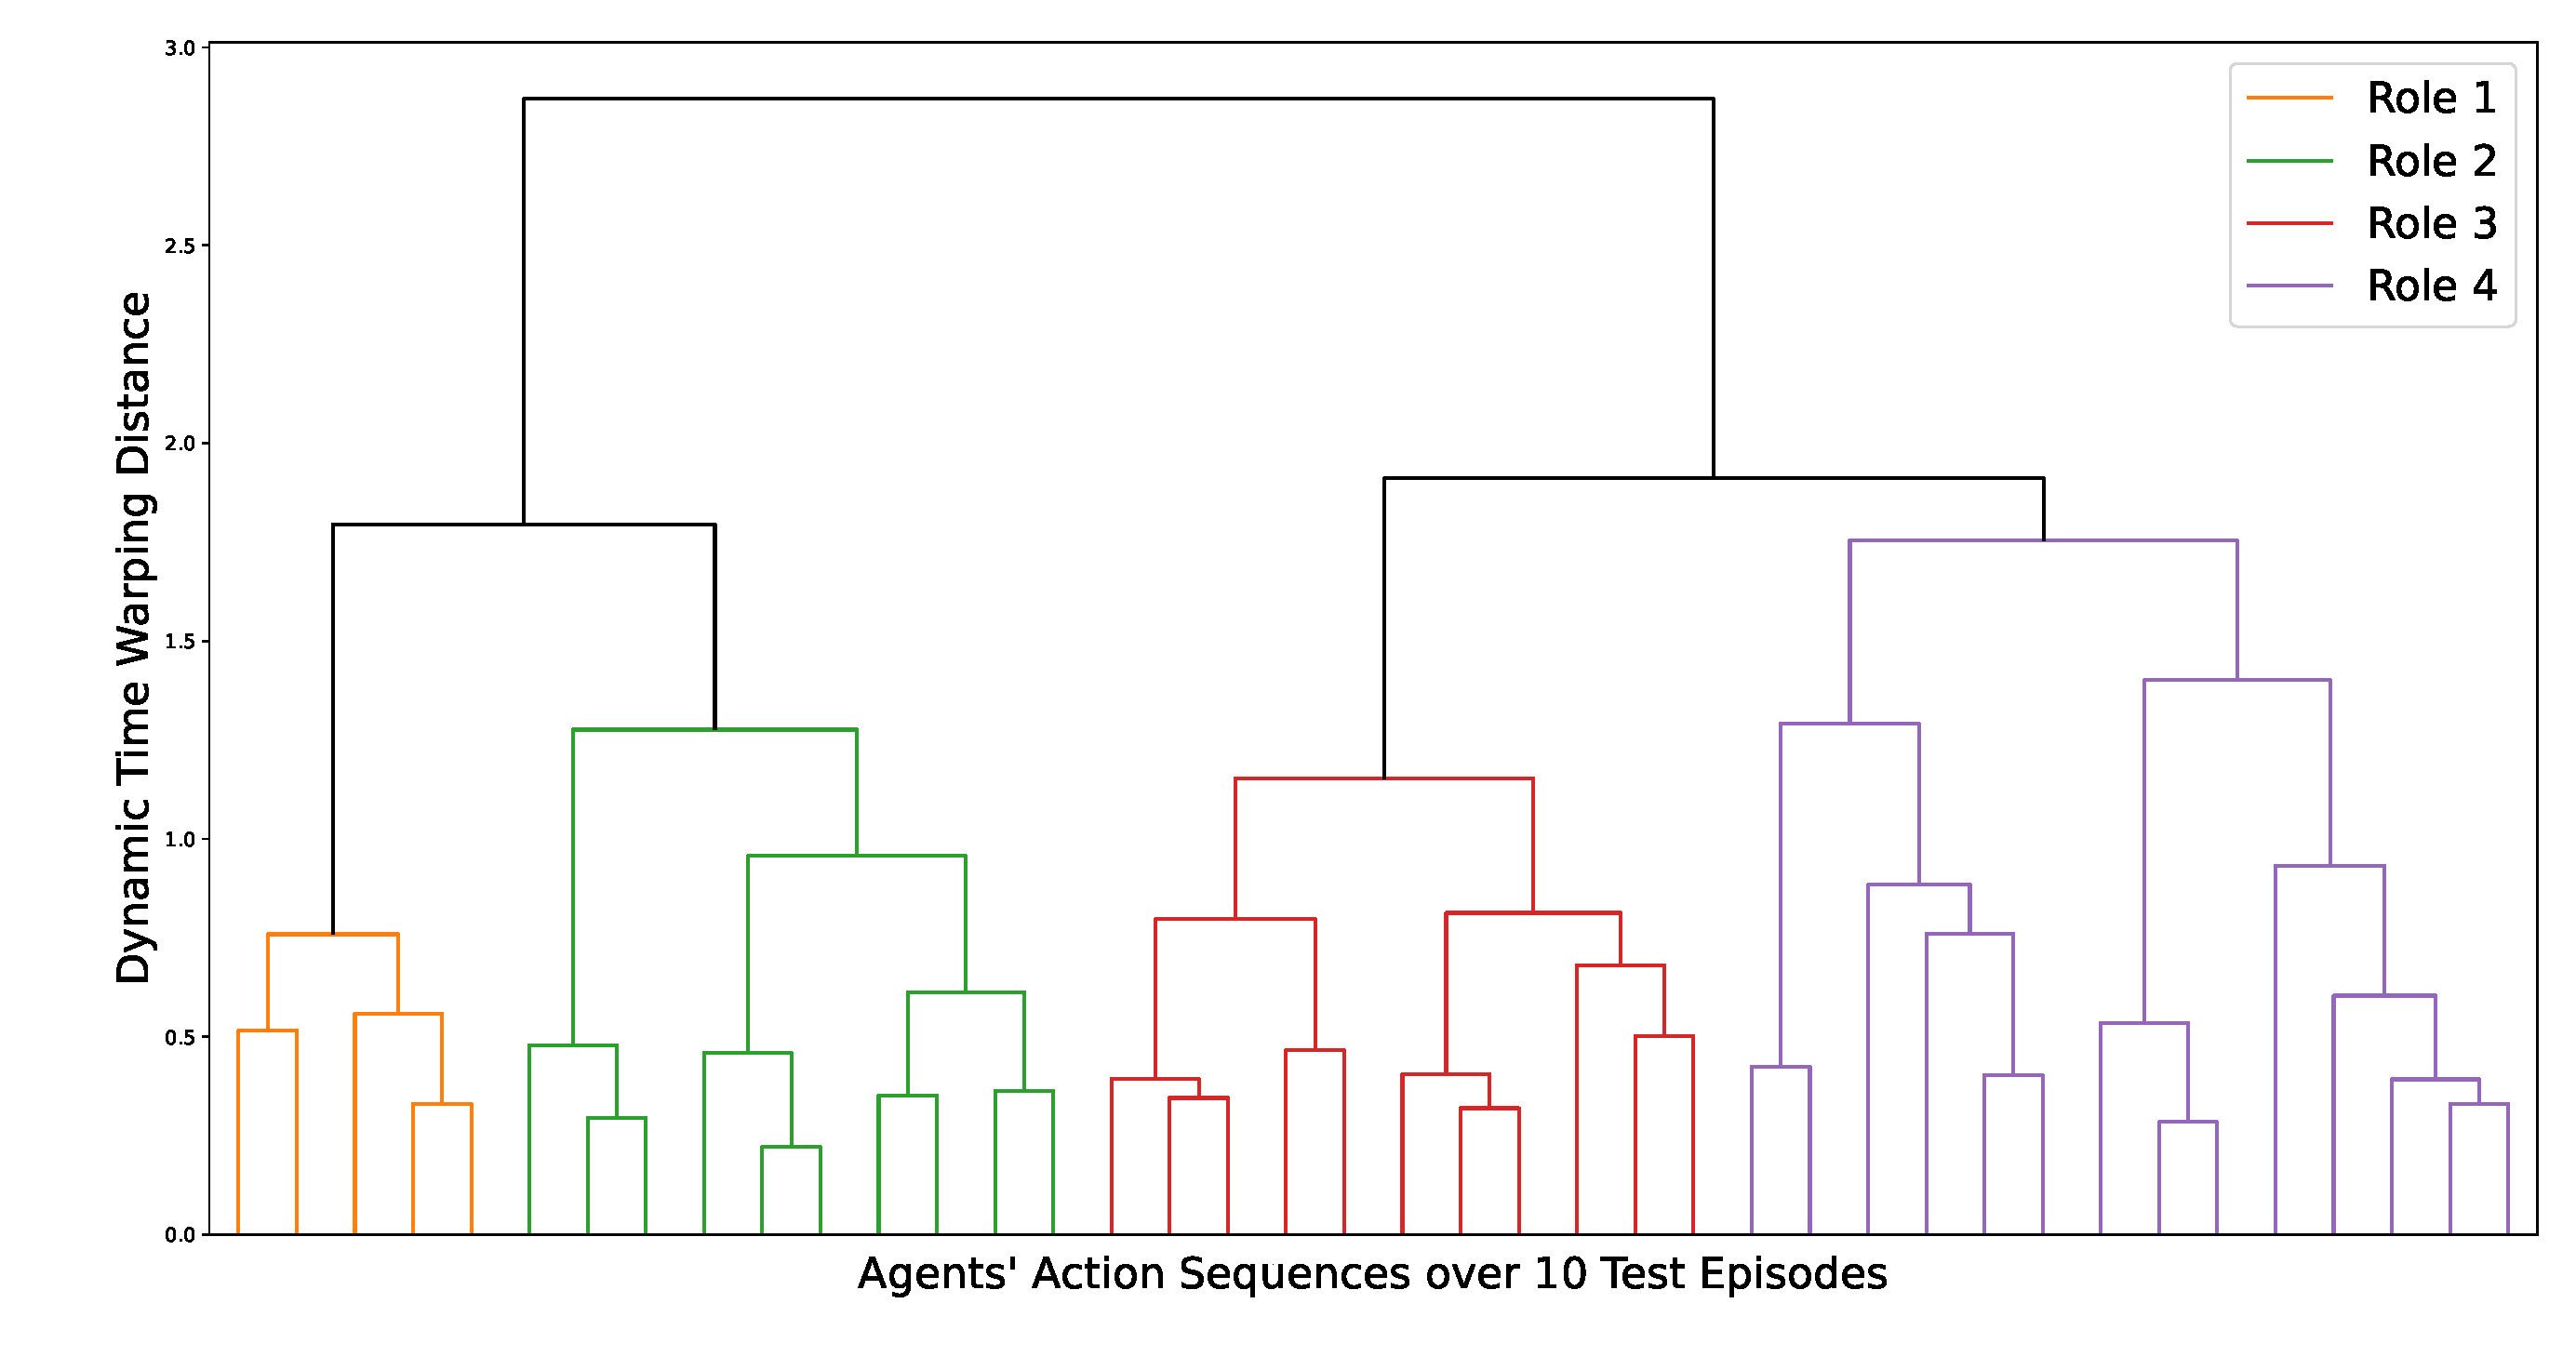
\includegraphics[width=0.49\textwidth]{figures/role_hierarchical_clustering.pdf}
  \caption{Dendrogramme obtenu après regroupement hiérarchique des trajectoires des agents pour l'inférence des rôles dans le scénario mixte.}
  \label{fig:trajectory_clustering_hrl}
\end{figure}

\begin{table}[h!]
  \centering
  \caption{Alignement des agents avec leurs rôles et missions.}
  \label{tab:alignment}

  {\footnotesize
    \begin{tabular}{>{\raggedright\arraybackslash}m{4.1cm}>{\centering\arraybackslash}m{1.5cm}>
      {\centering\arraybackslash}m{1.5cm}}
      \toprule
      \textbf{Référence}                                                           & \textbf{Score d'alignement (\%)} & \textbf{Pureté du regroupement (\%)} \\
      \midrule
      Multi-agents sans spécification organisationnelle                            & $\emptyset$                      & 62,7                                 \\
      Multi-agents avec spécifications organisationnelles souples                  & 85,3                             & 70,1                                 \\
      \textbf{Multi-agents avec spécifications organisationnelles rigides (KARMA)} & \textbf{96,2}                    & \textbf{89,4}                        \\
      \bottomrule
    \end{tabular}
  }
\end{table}

KARMA montre l'émergence de modèles comportementaux distincts alignés sur des rôles prédéfinis, ce qui valide le modèle organisationnel de KARMA et lui confère le score d'alignement le plus élevé (\textbf{96,2\%}), surpassant largement Multi-Agent w/o Org. Spec. (\textbf{85,3\%}), et démontrant ainsi la bonne coordination des comportements des agents. Dans les scénarios adversaires, la pureté du regroupement est la plus élevée pour KARMA, reflétant la différenciation claire des comportements des agents sous contraintes organisationnelles.
%
Des clusters distincts valident les comportements spécifiques à chaque rôle et soulignent l'interprétabilité des agents. Les références sans spécifications organisationnelles montrent une explicabilité réduite, comme en témoignent la pureté du regroupement et les scores d'alignement plus faibles avec des contraintes organisationnelles souples.

\subsection{Discussion générale}

Les résultats expérimentaux démontrent que KARMA comble efficacement plusieurs lacunes critiques de l'autoscaling Kubernetes. En intégrant MARL aux principes organisationnels, KARMA apporte des améliorations notables en matière de résilience opérationnelle, de robustesse face aux adversités et d'explicabilité. Sa capacité à décomposer des objectifs complexes en rôles et missions garantit un comportement coordonné des agents, comme en témoignent les taux de réussite élevés, les temps de récupération réduits et l'alignement sur les rôles prédéfinis observés dans tous les scénarios. L'utilisation d'un environnement de jumeau numérique, amélioré par un modèle de transition basé sur un MLP, renforce encore la capacité de KARMA à simuler des conditions réalistes, facilitant ainsi une formation robuste et une meilleure généralisation des politiques.

Cependant, KARMA n'est pas sans limites. Bien qu'il présente des progrès en matière d'adaptabilité, sa dépendance à l'expertise du domaine pour définir les rôles et les missions pourrait limiter son applicabilité dans les domaines où cette expertise est rare. En outre, la charge informatique requise pour la formation multi-agents et la modélisation de jumeaux numériques reste un défi pour les déploiements à grande échelle. Les résultats indiquent également que si KARMA réduit efficacement la latence et les demandes en attente, certaines références, telles que Rlad-core, offrent des performances comparables dans des scénarios spécifiques tels que la contention de ressources, mettant en évidence les domaines dans lesquels des améliorations pourraient être nécessaires.


\section{Discussion comparée des résultats}

\subsection{Discussion pour les scénarios non-orientés Cyberdéfense}
\label{sec:discussion_conclusion_future_work}

Le cadre MOISE+MARL présenté dans cet article vise à améliorer le contrôle et l'explicabilité dans MARL en intégrant des modèles organisationnels qui définissent des rôles et des missions explicites pour les agents. Les résultats expérimentaux obtenus dans plusieurs environnements indiquent que ce cadre aide les agents à adhérer aux comportements attendus tout en facilitant une meilleure convergence des politiques en limitant l'espace de recherche des politiques. Les résultats montrent également que les agents formés avec des rôles et des objectifs présentent des comportements très similaires à ceux déterminés via le cadre, ce qui suggère une cohérence entre l'application des spécifications organisationnelles et leurs effets attendus.

Cependant, la dépendance du cadre à des spécifications organisationnelles prédéfinies signifie qu'il peut avoir du mal à s'adapter à des environnements très dynamiques ou non structurés où les rôles et les missions des agents sont moins définis ou évoluent au fil du temps.
De plus, la charge informatique associée à l'application des contraintes organisationnelles et à la modification dynamique des récompenses et des actions peut poser des problèmes d'évolutivité. En outre, le TEMM peut être très gourmand en ressources informatiques, ce qui peut nuire à son applicabilité dans des scénarios en temps réel.

Nous poursuivons actuellement trois axes principaux :
%
% \begin{enumerate*}[label={\roman*)}, itemjoin={; \quad}]
\begin{itemize}
  \item Développer des mécanismes adaptatifs qui permettent aux rôles et aux missions d'évoluer de manière dynamique pendant la formation, afin que les agents puissent réagir aux changements en temps réel
  \item Explorer des méthodes automatisées, telles que les modèles linguistiques à grande échelle, pour générer des spécifications organisationnelles basées sur les comportements observés des agents afin d'aider les utilisateurs à définir manuellement ces spécifications
  \item Améliorer l'efficacité computationnelle du TEMM ou explorer d'autres méthodes d'évaluation pour des applications concrètes avec des populations d'agents plus importantes.
\end{itemize}

\subsection{Discussion pour le scénario d'infrastructure d'entreprise}

\noindent Nous avons proposé une modélisation Dec-POMDP des nœuds en réseau susceptibles d'être attaqués et défendus par des agents. Ce modèle vise à intégrer différents scénarios. La mise en œuvre de ce modèle a conduit à un simulateur dont certaines capacités ont été évaluées à travers un scénario MITRE ATT\&CK. À l'aide de trois approches, nous avons brièvement vérifié comment les approches par arbre de décision, aléatoire et par apprentissage par renforcement peuvent être appliquées à un agent à des fins de comparaison.
Soucieux de tirer parti de cette approche de simulation pour aborder des problèmes réalistes liés aux cyberdéfenseurs, en particulier dans le contexte de l'AICA, nous avons identifié les principales limites à surmonter :
automatiser l'intégration de scénarios plus réalistes en s'appuyant sur une base d'actions et de propriétés communes afin que les agents puissent explorer et agir comme dans des systèmes d'information apparemment similaires à la réalité~;
mettre en place un moyen d'utiliser les avantages des résultats obtenus avec les simulations pour des systèmes émulés ou réels tout en conservant les comportements des agents lors du déploiement~;
améliorer la coordination entre les agents, par exemple en créant plusieurs points d'entrée ou scénarios nécessitant une communication pour atteindre un objectif~;
et introduire de nouvelles contraintes dans les actions (telles que le coût, la durée d'exécution, etc.).


\subsection{Discussion pour le scénario d'essaim de drones}\label{sec:conclusion}

Notre contribution est motivée par le coût élevé de la conception de systèmes multi-agents de cyberdéfense (SMA) dans divers scénarios, en particulier lorsqu'il s'agit de faire face à des menaces en constante évolution. Pour remédier à ce problème, nous proposons un algorithme dédié appelé MAMAD, qui exploite l'apprentissage par renforcement multi-agents (MARL) en fonction des spécifications organisationnelles. MAMAD garantit le respect de certaines contraintes dans le comportement des agents, ce qui facilite la surveillance et la compréhension des agents formés.

MAMAD a été évalué à l'aide de notre implémentation PoC proposée pour le 3e défi CAGE, un scénario coopératif de cyberdéfense par essaim de drones conçu pour limiter/éliminer les programmes malveillants et leur impact. Nous avons établi divers modèles organisationnels, allant de modèles minimalement contraints à des modèles entièrement contraints. Nous avons évalué les stratégies collectives émergentes, affinées ou prédéfinies sur la base de critères de performance pendant et après la formation.

Les résultats indiquent que les modèles équilibrés en termes de contraintes, tels que le « modèle défensif actif », permettent d'obtenir un compromis significatif entre les contraintes et l'apprentissage autonome. Ce modèle utilise des règles prédéfinies simples pour détecter et traiter les menaces lorsque les observations sont sans ambiguïté, tout en permettant à l'agent d'apprendre à réagir dans d'autres scénarios.

Outre la contrainte des agents en fonction des spécifications organisationnelles, nous souhaitons prendre en compte des mécanismes d'explicabilité afin de comprendre les nouveaux modèles organisationnels appris. L'idée d'une amélioration itérative entre l'entraînement et l'explicabilité pourrait grandement bénéficier de l'apprentissage hiérarchique, qui aide à caractériser et à mettre en évidence les stratégies pendant l'apprentissage.
%En outre, si les premiers résultats obtenus avec LLM montrent qu'il s'agit d'un outil complémentaire prometteur pour MAMAD, il pourrait également offrir de nouvelles pistes pour expliquer les comportements collectifs, en particulier dans les scénarios de cyberdéfense où la plupart des environnements en réseau ne sont pas représentables de manière visuelle ou intuitive.

% Enfin, nous visons également à améliorer l'applicabilité de PRAHOM en développant des interfaces dédiées autour de PRAHOM afin de le rendre plus accessible aux contextes industriels et de recherche.


\subsection{Discussion pour le scénario d'architecture de microservices}
\label{sec:conclusion}
% Conclusion
%  - Résumé
%  - Résumé des points faibles et perspectives

Les résultats expérimentaux démontrent que KARMA comble efficacement plusieurs lacunes critiques de l'autoscaling Kubernetes. En intégrant MARL à des principes organisationnels, KARMA améliore la robustesse face à l'adversité et l'explicabilité. Sa capacité à décomposer des objectifs complexes en rôles et missions garantit un comportement coordonné des agents. L'utilisation d'un modèle de transition basé sur MLP renforce encore la capacité de KARMA à simuler des conditions réalistes.
%
% Les principales contributions de ce travail sont les suivantes :
% \begin{itemize}
%     \item \textbf{Environnement de jumeau numérique :} un modèle de simulation réaliste et représentatif dérivé de traces de clusters, permettant un apprentissage sûr et efficace des politiques grâce à un jumeau numérique.
%     \item \textbf{Conception guidée par l'organisation :} L'utilisation de rôles et de missions pour décomposer la résilience opérationnelle en sous-objectifs gérables, fournissant une méthode systématique pour la coordination et la prise de décision des agents.
%     \item \textbf{Apprentissage par renforcement multi-agents (MARL) :} exploitation des algorithmes MARL pour former les agents de manière collaborative, garantissant l'adaptabilité et la robustesse dans des scénarios complexes à objectifs multiples.
%     \item \textbf{Explicabilité et analyse :} Analyse des comportements des agents à l'aide du regroupement des trajectoires et de la détection des interactions entre agents, améliorant ainsi l'interprétabilité et la confiance dans les décisions des agents.
%     \item \textbf{Gestion de scénarios adverses :} Démontrer la résilience du cadre proposé dans des scénarios tels que les attaques DDoS, qui sont critiques pour la fiabilité des systèmes cloud natifs.
% \end{itemize}
%
% \

Cependant, certains aspects doivent être approfondis :
\begin{enumerate*}[label=\textbf{\arabic*)}, itemjoin={;\quad }]
  \item \textbf{Écart entre la simulation et la réalité :} Même si nous générons un modèle de simulation quasi réaliste à partir des traces de l'environnement, nous devons mieux simuler les défaillances imprévues du système qui n'ont pas été prises en compte
  \item \textbf{Dépendance à l'expertise du domaine :} La définition des rôles, des missions et des structures de récompense repose fortement sur des connaissances spécifiques au domaine, ce qui peut limiter la généralisation du cadre
  \item \textbf{Surcharge informatique :} Le processus d'entraînement avec des configurations multi-agents et des contraintes organisationnelles nécessite des ressources informatiques importantes.
  \item \textbf{Évolutivité vers des clusters multi-nœuds :} Bien que les expériences actuelles se concentrent sur un cluster à nœud unique, des évaluations préliminaires sont en cours sur des déploiements à plus grande échelle.

  % \item \textbf{Sensibilité aux variations de la charge de travail :} Bien que KARMA fasse preuve d'adaptabilité, des changements brusques dans les modèles de charge de travail ou les configurations de clusters peuvent nécessiter un réentraînement ou un ajustement des politiques des agents.
  % \item \textbf{Portée de l'évaluation :} Bien que le cadre ait été testé dans divers scénarios, y compris dans des conditions adverses, ses performances sur des clusters plus grands et plus hétérogènes restent à valider.
\end{enumerate*}


% Bien que KARMA ne soit pas une solution universelle à tous les défis liés à l'autoscaling dans Kubernetes, il constitue une avancée dans la résolution des principales lacunes en matière de résilience opérationnelle, d'adaptabilité et d'explicabilité. La combinaison du MARL et des principes organisationnels du cadre offre une base prometteuse pour la recherche et le développement futurs.

\subsection{Synthèse comparative}

L’ensemble des scénarios expérimentaux présentés — qu’ils soient abstraits (Overcooked, Predator-Prey), sectoriels (infrastructure d’entreprise, drones, microservices) ou réalistes (cyberdéfense MITRE) — permet d’évaluer la portée et les limites du cadre MOISE+MARL à travers des contextes variés. Cette diversité constitue un levier précieux pour dégager des invariants et des facteurs de succès de l’approche.

\paragraph{Couverture des critères.} Dans tous les scénarios, le cadre permet d’adresser les critères d’autonomie (C1), de couverture fonctionnelle (C2) et d’adaptation (C3), en facilitant l’entraînement de politiques coordonnées dans des contextes dynamiques. Les agents sont capables d’explorer des solutions coopératives pertinentes, même lorsque l’environnement est complexe ou incertain.

En revanche, les critères liés à la sûreté (C4), l’explicabilité (C5), la résilience (C6) ou la soutenabilité (C8) dépendent fortement des spécifications organisationnelles fournies. Par exemple :
\begin{itemize}
  \item Le critère C4 (sûreté) est bien représenté dans les scénarios microservices et drones, grâce à l’imposition explicite de restrictions dans les règles de rôle.
  \item L’explicabilité (C5) est particulièrement travaillée dans le scénario Overcooked via le module d’analyse TEMM, mais plus difficile à interpréter dans des contextes cyber-réalistes.
  \item La résilience (C6) est atteinte lorsqu’une redondance fonctionnelle ou des mécanismes de relais sont encodés dans les missions.
  \item La soutenabilité (C8) reste peu explorée, mais pourrait être abordée en intégrant des métriques énergétiques ou des contraintes sur l’obsolescence logicielle.
\end{itemize}

\paragraph{Spécificités par scénario.}
\begin{itemize}
  \item Les environnements non-cyber (Overcooked, Predator-Prey) illustrent bien la capacité du cadre à structurer un apprentissage organisationnel, mais dans des contextes abstraits, sans cybermenace ou contraintes de sécurité réelles.
  \item Le scénario d’infrastructure d’entreprise introduit des dynamiques plus proches du monde réel, mais reste limité par la difficulté d’une simulation fine et la complexité de coordination dans un système ouvert.
  \item Le scénario drone permet d’illustrer l’importance de la structure organisationnelle pour garantir une réponse cohérente à des menaces distribuées, et souligne la complémentarité entre règles fixes et comportements appris.
  \item Le scénario microservices met en lumière le potentiel du cadre pour des systèmes cloud-natifs autonomes et adaptatifs, mais révèle aussi les limites en termes de généralisation et de coût computationnel.
\end{itemize}

\paragraph{Éléments transversaux.} Trois enseignements clés émergent de cette comparaison :
\begin{enumerate}
  \item \textbf{La spécification organisationnelle est un levier essentiel} pour orienter l’apprentissage vers des solutions sûres et compréhensibles, à condition qu’elle soit bien adaptée au contexte.
  \item \textbf{L’analyse post-apprentissage (via TEMM ou équivalent) est indispensable} pour assurer une boucle de validation organisationnelle et guider la reconfiguration des rôles ou missions.
  \item \textbf{Le coût computationnel reste un facteur limitant} dans les scénarios à forte dimensionnalité ou population, appelant à des méthodes d’optimisation, de distillation ou de modularisation futures.
\end{enumerate}

\

De manière synthétique, la méthode proposée démontre une capacité robuste à produire des politiques respectueuses de contraintes complexes et à rendre les comportements émergents plus lisibles. Elle s’adapte à des contextes variés, mais appelle encore des efforts pour traiter pleinement les critères C5 (explicabilité), C6 (résilience) et C8 (soutenabilité) de manière généralisée.


\clearpage
\thispagestyle{empty}
\null
\newpage


\chapter*{Conclusion}
\addcontentsline{toc}{chapter}{\textbf{Conclusion}}

Cette partie a permis de valider expérimentalement la méthode \acn{MAMAD} à travers des scénarios simulés, couvrant des contextes variés de conception de systèmes multi-agents : infrastructure d’entreprise, essaim de drones, et orchestration de microservices. À chaque étape du pipeline proposé, l’implémentation via la plateforme \acn{CybMASDE} a démontré la faisabilité de l’approche, tout en soulignant les apports spécifiques du couplage MOISE+ avec l’apprentissage multi-agent.

Les résultats obtenus montrent des gains notables en termes d’autonomie, de résilience et de conformité organisationnelle des agents. L’analyse comparative entre les versions « guidées » et « non guidées » par l’organisation a permis d’évaluer l’impact de chaque composant de la méthode, à la fois sur les performances observées et sur la capacité à extraire des spécifications émergentes cohérentes. Les métriques introduites (comme le SOF ou le FOF) ont apporté une lecture inédite des comportements collectifs, en reliant les trajectoires apprises aux objectifs structurels du système.

Malgré ces résultats encourageants, plusieurs limites ont été identifiées : dépendance aux environnements simulés, couverture partielle des contextes applicatifs, et nécessité de ressources computationnelles importantes. Ces éléments seront discutés plus en détail dans la dernière partie de ce manuscrit, qui propose un retour réflexif sur l’ensemble de la démarche entreprise.

\vspace{1em}

\noindent
Dans la suite, nous procéderons à une synthèse des contributions, discuterons les limites de la méthode, et ouvrirons des perspectives sur son extension future, tant en recherche qu’en application.
